\documentclass{ufpatcc}

\include{include}
%% Packages used for the TCC

%\usepackage{booktabs}

%%%% Definitions and New commnads %%%%

\newcommand{\sen}{\operatorname{sen}}
\newcommand{\mbeq}{\overset{!}{=}}

\renewcommand\Re{\operatorname{Re}}
\renewcommand\Im{\operatorname{Im}}

%%%% New control sequences %%%%

\newcommand{\redeq}[1] {\textcolor{red}{#1}}
\newcommand{\blueeq}[1] {\textcolor{blue}{#1}}
\newcommand{\att}[1] {\textcolor{red}{#1}}
% Used Packages:
\usepackage{tikz}
\usepackage{float}
\usepackage{steinmetz}
\usetikzlibrary{arrows,shapes,shapes.multipart}
%\usepackage[brazil]{babel}
\usepackage[T1]{fontenc}
\usepackage[utf8]{inputenc}
\usepackage{amsmath}
\usepackage{amsfonts}
\usepackage{enumitem} % To adjust lists
\usepackage{verbatim} % Multi-line comments
\usepackage{mathabx} % Package that contains the circular convolution symbol
\usepackage{graphicx}
\usepackage{caption}
\usepackage{subcaption}
\usepackage{units}
\usepackage{adjustbox}
\usepackage{dirtytalk}

%\usepackage[backend=bibtex8]{biblatex}

\ifpdf

\ifdefined\hyperref
\else
\usepackage[pdftex,colorlinks]{hyperref}
\fi

\hypersetup{%
pdftitle={Some title},
pdfauthor={Your name - LaPS - UFPA},
pdfkeywords={DSP,Signal},
pdfstartview={FitH}, %% <--
urlcolor=black,
%linkcolor=blue,
linkcolor=black,
%citecolor=red,
citecolor=black,
}

% Ensiar o Latex a separar silabas
\hyphenation{DMT En-ge-nhei-ro}


\ufpaTitulo{An FPGA-Based Radion Frontend for LTE Transmission on Cloud RAN}

\ufpaAutor{Gabriel Peixoto de Carvalho}
\ufpaSegundoAutor{}
\ufpaOrientador{Prof. Aldebaro Barreto da Rocha Klautau Junior}
\ufpaCoordenadorCurso{Prof. Jos\'{e} Augusto de Lima Barreiros}

\ufpaCoOrientador{Prof. Wilson Pacheco Ferreira}
\ufpaMembroBancaA{Prof. Francisco Carlos Bentes Frey Muller}
\ufpaMembroBancaB{Eng. Igor Mesquita de Almeida}


\begin{document}

\ufpaPaginaDeRosto

\ufpaPagRostodo

\ufpaPaginaDeAprovacao

%%%%%%%%%%%%%%%%%%%%
%   Oferecimento   %
%%%%%%%%%%%%%%%%%%%%

\begin{ufpaOferecimento}
\index{Oferecimento@Oferecimento}%
\addcontentsline{toc}{chapter}{Dedicat�ria}

\end{ufpaOferecimento}

%%%%%%%%%%%%%%%%%%%%
%  Agradecimento   %
%%%%%%%%%%%%%%%%%%%%

\begin{ufpaAgradecimentos}
\index{Agradecimentos@Agradecimentos}
\addcontentsline{toc}{chapter}{Agradecimentos}

\begin{flushright}
Gabriel Peixoto de Carvalho
\end{flushright}

\end{ufpaAgradecimentos}

%%%%%%%%%%%%%%%%%%%%
%      Ep�grafe     %
%%%%%%%%%%%%%%%%%%%%

\begin{ufpaEpigrafe}
Viva como se voc� fosse morrer amanh�. Aprenda como se voc� fosse viver para sempre.\\
\begin{flushright}Mahatma Gandhi\end{flushright}
\end{ufpaEpigrafe}

%%%%%%%%%%%%%%%%%%%%%
%  Lista de Siglas  %
%%%%%%%%%%%%%%%%%%%%%

\chapter*{Lista de Siglas} \label{sec:siglas}
\begin{enumerate}
 \item ADSL - \textit{Linha de assinante digital assim�trica}
 %\item AWGN - \textit{Ru�do aditivo branco Gaussiano}
 %\item BER - \textit{Taxa de erro de bit}
 %\item DFT - \textit{Transformada de Fourier discreta}
 %\item DMT - \textit{Multi-tom discreto}
 %\item DSL - \textit{Linha de assinante digital}
 %\item FEQ - \textit{Equalizador em frequ�ncia}
 %\item FFT - \textit{Transformada rápida de Fourier}
 %\item FTTH - \textit{Fibra até a residência}
 %\item G.fast - \textit{Acesso rápido aos terminais do assinante}
 %\item ICI - \textit{Interferência inter-portadora}
 %\item IDFT - \textit{Transformada de Fourier discreta inversa}
 %\item IFFT - \textit{Transformada rápida de Fourier inversa}
 %\item ISI - \textit{Interferência inter-simbólica}
 %\item OFDM - \textit{Modulação por divisão ortogonal de frequência}
 %\item PC - \textit{Prefixo cíclico}
 %\item PSD - \textit{Densidade espectral de potência}
 %\item RIC - \textit{Resposta impulsiva do canal}
 %\item SC - \textit{Sufixo cíclico}
 %\item SER - \textit{Taxa de erro de símbolo}
 %\item SNR - \textit{Razão sinal ruído}
 %\item VDSL - \textit{Linha de assinante digital com taxa de bit muito alta}
 %\item 4GBB - \textit{Quarta geração de banda larga}
\end{enumerate}
 


\chapter*{Lista de S�mbolos} \label{sec:simbolos}
\begin{description}[labelsep=5em, align=left,labelindent=2cm]
\item[$b$] Taxa agregada de bits alcancavel para o sistema
%\item[$f_s$] Frequência de amostragem
%\item[$H(f)$] Espectro do canal
%\item[$H_k$] Ganho do $k$-ésimo subcanal
%\item[$\mathbf{ H_\text{ICI}}$] Matriz de ICI no domínio do tempo
%\item[$\mathbf{ H_\text{ISI}}$] Matriz de ISI no domínio do tempo
%\item[$L$] Dispersão do canal
%\item[$n$] Índice da amostra
%\item[$n_0$] Indice da amostra de início do símbolo recebido para o receptor sincronizado
%\item[$N$] Número de pontos da DFT ou tamanho do vetor símbolo DMT
%\item[$N_a$] Número de amostras afetadas por ISI e ICI
%\item[$p_k$] Parte real do $k$-ésimo subsímbolo
%\item[$P_x$] Potência total de transmissão
%\item[$q_k$] Parte imaginária do $k$-ésimo subsímbolo
%\item[$\mathbf{Q}$] Matriz DFT
\end{description}


%%%%%%%%%%%%%%%%%%%%%%%%%%%%%%%%%%%%%%%%%%%%
%  Insere a lista de Figuras e de Tabelas  %
%%%%%%%%%%%%%%%%%%%%%%%%%%%%%%%%%%%%%%%%%%%%

\listoffigures \clearpage \listoftables \clearpage

%%%%%%%%%%%%%%%%%%%%
%      Sum�rio     %
%%%%%%%%%%%%%%%%%%%%

\tableofcontents    \clearpage

%%%%%%%%%%%%%%%%%%%%
%      Resumo      %
%%%%%%%%%%%%%%%%%%%%

\begin{ufpaResumo}


\end{ufpaResumo}

\begin{abstract}
    
The evolution of mobile services in terms of access technologies and application 
layers is driving a huge change in mobile communication systems. A recent hot 
topic in the field is the rise of the cloud computing paradigm, thus the idea 
known as cloud radio access networks (Cloud-RAN) is growing in the industry. 
This behavior comes from the potential of cloudification for improvement in the 
efficiency of resource allocation, manageability and power consumption, aspects 
inherent of traditional RANs.\\

Thus, with the emerging of C-RAN, several questions about how to implement and 
which tools to use come naturally. This work aims to evaluate the potential of a 
programmable fronthaul radio interface, as known, actual network does not have 
the adaptative capability needed for the C-RAN. For this work a setup of a radio 
unit, composed by two fpgas (one acting as the Baseband unit and other as the
(digital front-end) of the radio unity) connected through ethernet and two 
transceivers (analog front-end), one in each FPGA. Within this setup various 
algorithms can be tested and can be evaluated in LTE scenarios because the 
transceiver works in LTE and C-RAN .\\

This work shall focus on the evaluation of the radio interface and perform the 
tests inherent to it, exploring FPGA adaptability and parallelism with the 
internal and external communication protocols, and so exploring the advantages 
of the transceiver used, the fmcomms2  development board (AD9361 chip) from 
Analog devices, which is a device broadly used in software defined radio 
hardwares, as known as USRPs (Universal Software Radio Peripheral). \\

An aspect of the transceiver that is very attractive to the C-RAN paradigm is 
its configurability and scalability, capable of real-time adjustments in the 
sampling frequency or operation mode from 2x2 to 4x4 MIMO (Multiple Inputs and 
Multiple Outputs), this real-time adaptive characteristic is ideal to C-RAN 
environment.\\

The results are generated primarily aiming a fidelity in the transmitted and 
receiver signals, after these results are conclusive it is possible to proceed 
to more complex tests and approaches of this setup. Another test made was the 
analysis of the synchronization between  receiver and transceiver using a CIPRI 
emulator implemented in FPGA logic, which is the standard fronthaul interface, 
in this test it is possible to observe the advantages of the programmable radio 
front-end in the system.\\



\end{abstract}

%%%%%%%%%%%%%%%%%%%%%
%   Corpo do TCC    %
%%%%%%%%%%%%%%%%%%%%%

\pagenumbering{arabic}

\part{Introduction}
\chapter{Introduction}
\label{chap:intro}

%The world is much more interconnected and the economy is growing wilder and
%wilder, a lot of economical issues rise in different countries almost every
%year. The climate changes are also a concern to the modern governments, thus the
%idea of re-utilizing resources and  make these resources be more economically
%and environmentally friendly are a goal for modern research and development.

The scalability and reconfigurability of telecommunication systems is very
interesting for the companies and operators in the current economic needs,
re-utilization is the key to decrease deployment and equipment update. This work
aims to evaluate the feasibility of a radio-fronthaul System for
\textit{Long-Term Evolution} (LTE) transmissions in a reconfigurable and scalable
environment of \textit{Cloud Radio Access Network} (CRAN).

Cloud computing is a paradigm which use is getting more common in companies and
developers, it solves some infrastructure problems of small and big companies.
Companies do not need to own computers or anything locally to operate,
everything can be done remotely and a more experienced company and staff can
offer such infrastructure or application as a service. Such idea of having
everything as a service is very attractive both economically  and
environmentally because there is no waste of resource, everything is scalable to
the need of the client and upgradeable if needed.

The Radio access technologies have been evolving from audio traffic to intensive
data traffic over the recent standards, because the mobile devices got a myriad
of functions which could only be executed by \textit{Personal Computers} (PC).
Such networks demand a huge amount of resources. Hence, there are concerns about
how to develop and deploy these networks such as backwards compatibility of the
devices, because an operator would never deploy a network which is not
compatible with previous standards equipments, this is not profitable. Having
these ideas in mind the C-RAN concept began to be developed,  where the
resources for the RANs are scalable and configurable to needs of the clients and
operators, and where the baseband processing is all done on the cloud and the
radio frontends are reconfigurable to handle different data and modulation
outputs.

The reconfigurable fabric of the \textit{Field Programmable Gate Array} (FPGA)
technology is very attractive to implement such radio front-ends and other
reconfigurable computing tasks, because it is flexible to be reconfigured
on-the-run, offers a really good parallel processing and I/O capabilities. Thus
this work aims to evaluate the implementation feasibility of a radio frontend
LTE transmissions in a Cloud RAN environment (adaptability and
reconfigurability).

This work is implemented in a Xilinx Virtex 7 FPGA and using the transceiver
board \textit{FMCOMMS2} from \textit{Analog Devices}, this transceiver can be
reconfigured in real time and runs up to 6 GHz band, it has been chosen because
of such reconfigurability properties.

The remainder of this text is organized in 4 parts as follows:

Part II is a literature review of some theoretical background used in this work
development, divided in three chapters. Chapter \ref{chap:sdr} offers an
overview of Cloud and Software defined radio, because reconfigurability and
scalability are features desired in SDR field and in this work. In Chapter
\ref{chap:lte} there is an overview in Digital Communication Systems and LTE,
since this work shall focus on LTE  frequency band transmissions.

Part III is the core of the work, Chapter \ref{chap:implementation} describes
the implementation of this work's setup and gives an overview of functionalities
of both FPGA and Fmcomms2 shall be explained. The development will be described
in terms of how it was implemented in both FPGA logic and software drivers.

Part IV reports all the results of this work in Chapter
\ref{chap:results}. The configuration results report how the transceiver board
communication and configuration were done. The simulation results aim to show
the VHDL blocks simulation prior to hardware implementation and at last the
transmission results aim in report the integrity of the transmitted signals.

Part V presents the conclusions and future works in Chapter
\ref{chap:conclusion}, which aim to report everything learned from this work and
what can be done to improve the transmission/reception quality.

\part{Literature Review}
\chapter{Synchornization}

\section{Carrier Recovery}

Carrier recovery is a process used in coherent demodulation where the phase
and the frequency of the transmitter carrier wave are recovered by the receiver
and thus after having such information it is possible to extract the information
in the transmitted signal.\\
Considering that the phase and frequency of the transmitted wave probably will
be affected by noise, it is not a straight-forward method, it includes filtering
and usually feedback systems to correct the erros in phase or frequency caused
by the noise.\\
This chapter aims in the brief exploration of some techniques used for carrier
recovering, such as Phase locked loops, costas loop and others.\\

\subsection{Costas Loop}

\part{Implementation}
\chapter{FMComms2}
\section{AD9361}
\label{sec:ad9361}

The AD9361 is a high performance RF transceiver. Its programmability and adaptability makes it ideal for a wide range of transceiver applications. This device combines a RF front end with a flexible and configurable mixed-signal baseband section and frequency synthesizers, simplified configuration digital interface to a processor. 
The AD9361 operates from 70 MHz to 6.0GHz range with supported channel bandwidths from 200 KHz to 56 MHz and the AD9361 is a 2 Rx and 2 Tx device packed in a 10mm x10mm, 144 ball chip package ball grid array (CSP\_BGA).

\subsection{General Description}

AD9361 is a highly integrated RF frequency transceiver capable of being configured for a wide range of applications, including 3g and 4g frequency applications. AD9361 and AD9364 almost the same hardware and specifications, the difference is that AD9361 is a 2x2 MIMO and AD9364 is a 1x1 \cite{ad9361_wiki}.
The programmability allows the AD9361 to be operated in Frequency Division Duplex (FDD) and Time Division Duplex (TDD) systems, allowing this transceiver to operate in a variety of communication standards. Another interesting feature is the capability of integration with a wide range of BBPs (Baseband Processors) using a single or dual 12-bit parallel data port or a 12-bit LVDS (Low voltage Differential signaling), which uses the FMC connector in the FMCommS2 \ref{sec:fmcomms2}.
AD9361 also provides self-calibration and automatic gain control (AGC) systems to maintain good performance under variable conditions, such as temperature and signal quality. The transceiver has also various modes of test mode with the Built-in Self Test (BIST) modes which can be used for the designers to debug desgs during prototyping.
This configurability and adaptability is very attractive for Software Defined Radio (SDR) and for C-RAN systems, indeed ad9361 is already being used in some Universal Software Radio Peripheral (USRP) from ettus research (National Instruments), this alone is a proof that AD9361 can work in a wide range of systems and standards.

\begin{figure}[htbp]
    \centering
    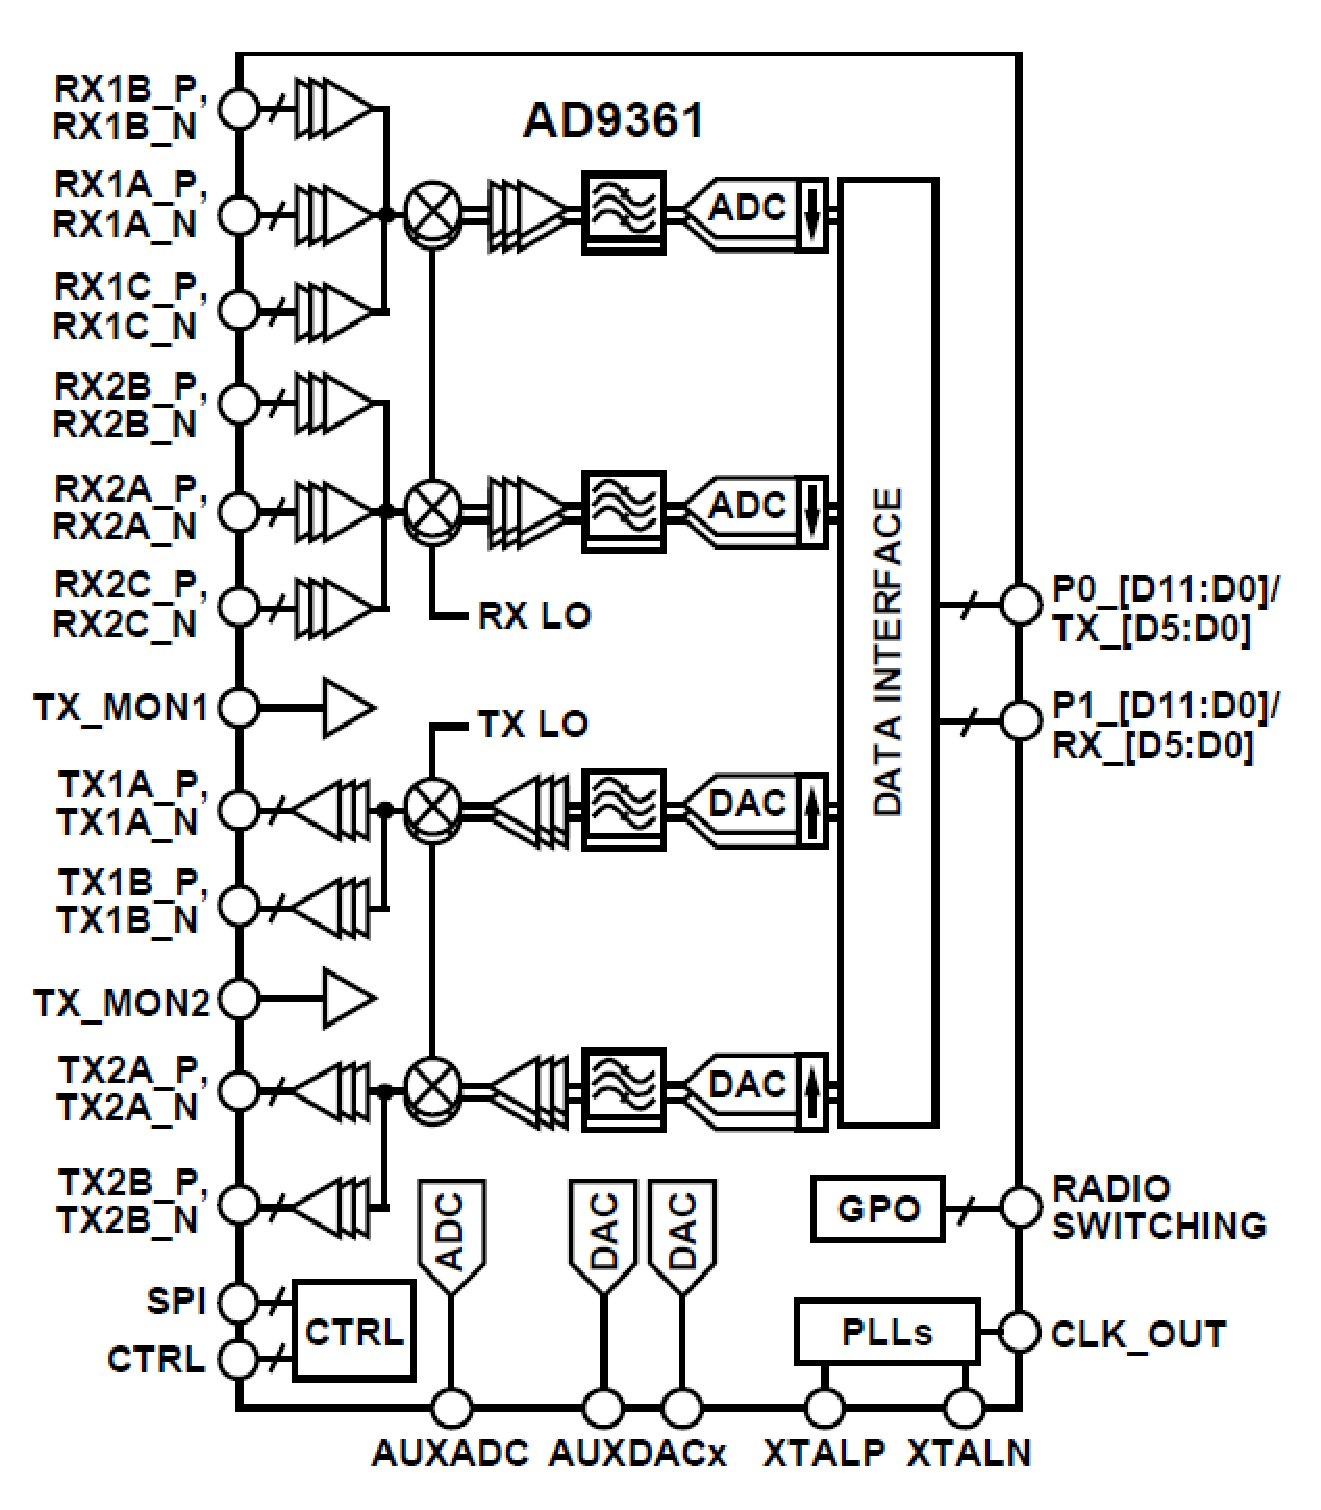
\includegraphics[width=0.65\textwidth]{./figures/ad9361_functional_diagram}
    \caption{ AD9361 Functional Block Diagram
    \label{fig:ad9361func}}
\end{figure}

\subsection{Receiver}

The receiver section has all the blocks necessary to receive analog RF signals and convert them to digital data which can be used by the BBP. there are two independently controlled channels that share same frequency synthesizer. This characteristic makes possible to the AD9361 to operate in MIMO systems.

Each channel has 3 inputs which can be multiplexed into the signal chain, making possible to use the AD9361 into systems with multiple antenna inputs. The Receiver is a direct conversion system that contains a Low noise amplifier (LNA) , followed by a matched in-phase and quadrature amplifier, mixers, and band shaping filters that down convert received signals to baseband for digitization. External LNAs can also be interfaced to the AD9361 allowing more flexibility in the design.
The receiver signal path passes downconverted signals (I and Q), which are schematically identical to each other,  to the baseband (BB) receiver section. The BB section is composed by two programmable low-pass filters, with programmable corner frequency for each filter, 12-bit ADC and four stages of decimating filters, each of the four decimation filters can be bypassed. 
The gain control is achieved by a preprogrammed gain index map, a lookup table for example, this map distributes gain in order to achieve optimal performance at each level. This optimal behavior can be achieved by enabling AGC, which can run in two modes, fast and slow gain control. This allow for the BBP to make gain adjustments as needed.
Each channel also contains independent RSSI measurement capability, DC offset tracking and all other circuitry needed for self-calibration.

The receiver ADC is a 12-bit sigma-delta ($\Sigma-\Delta$) ADC which allows adjustable sample rates. This ADC produces data streams from the received signals and such digitalized signals can be conditioned further by a series of decimation filters and a 128-tap FIR filter with additional decimation settings.
The sampling rate of each digital filter is adjustable through changes in the decimation factors to produce the needed data rate.

In short, the Receiver chain has:

\begin{itemize}
	\item LNA - Low noise Amplifier
	\item Matched in-phase amplifier;
	\item Quadrature Amplifier;
	\item Band Shaping Filters;
	\item Analog low pass filters;
	\item 12-bit DAC;
	\item 4 stages of decimation filters (128-tap FIR filters);
	\item Automatic gain Control;
\end{itemize}

\begin{figure}[htbp]
    \centering
    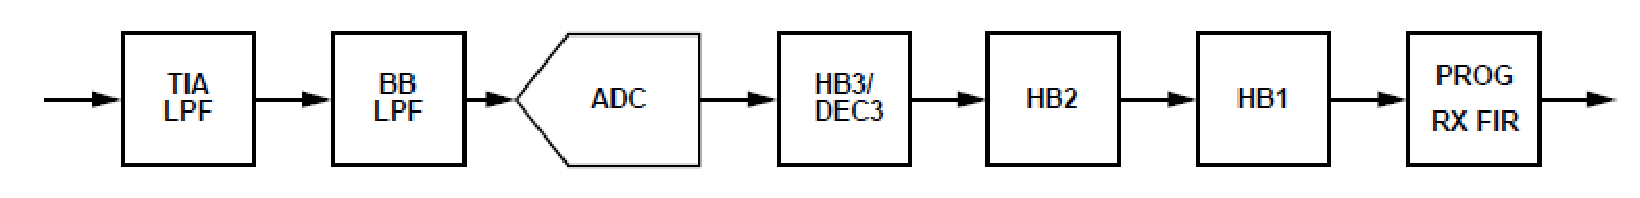
\includegraphics[width=0.65\textwidth]{./figures/rx_chain}
    \caption{ Receiver Signal Path
    \label{fig:rxchain}}
\end{figure}


\subsection{Transmitter}

Like the receiver section, the transmitter section contains two identical and independently controller channels, which share the same frequency synthesizer,  that provide all digital signal processing, mixed signal and RF blocks necessary to implement a direct conversion system from digital data to RF.
The Tx signal path receives from the BBP 12-bit 2s complement I-Q format data in the digital interface and each channel goes through a 128-tap FIR filter with interpolation options, which is fully programmable. Then the signal goes through a series of additional interpolation filters that manipulates the signal with additional filtering and data rate interpolation before reaching the 12-bit DAC, note that all these filtering and interpolation steps can be bypassed if desired.
Each 12-bit DAC has an adjustable sampling rate and its analog output passes through to low pass filters to remove any sampling artifacts before going to the RF mixer, these low pass filters corner frequencies can be programmable too. After all these filtering and analog conversion steps, the I and Q signals are recombined and modulated in the carrier frequency, which can be adjusted by changing the synthesizer frequency. These analog combined signals passes through additional analog filters for better band shaping and then it can be transmitted to the output amplifier. Each Transmitting channel provides wide attenuation adjustment range with fine granularity in order to optimize SNR.

\begin{figure}[htbp]
    \centering
    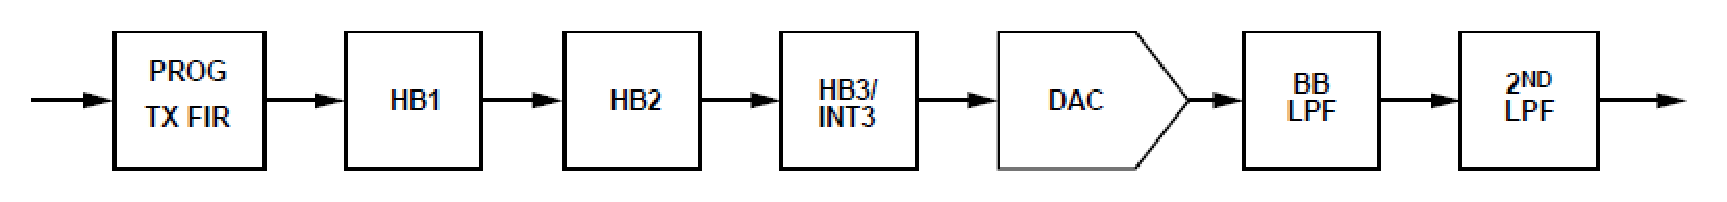
\includegraphics[width=0.65\textwidth]{./figures/tx_chain}
    \caption{ Transmitter Signal Path
    \label{fig:txchain}}
\end{figure}


Identical to the receiver chain, the transmitter chain has also built-in self-calibration circuitry into each transmitting channel providing an automatic real-time adjustment. The transmitter also provides a TX monitor block for each channel, this block monitors the transmission output and routes it back through an unused receiver channel to the BBP for signal monitoring, but these monitoring option is only available in TDD mode operation while the receiver is idle.

In short the transmission chain has:

\begin{itemize}
	\item 128-tap FIR filters;
	\item Interpolation Filters;
	\item 12-bit DAC;
	\item Analog Low-pass Filters;
	\item Additional band shaping analog filters;
	\item Attenuation adjustment;
	\item self-calibration circuits;
	\item Tx signal Monitor.
\end{itemize}

\begin{figure}[htbp]
    \centering
    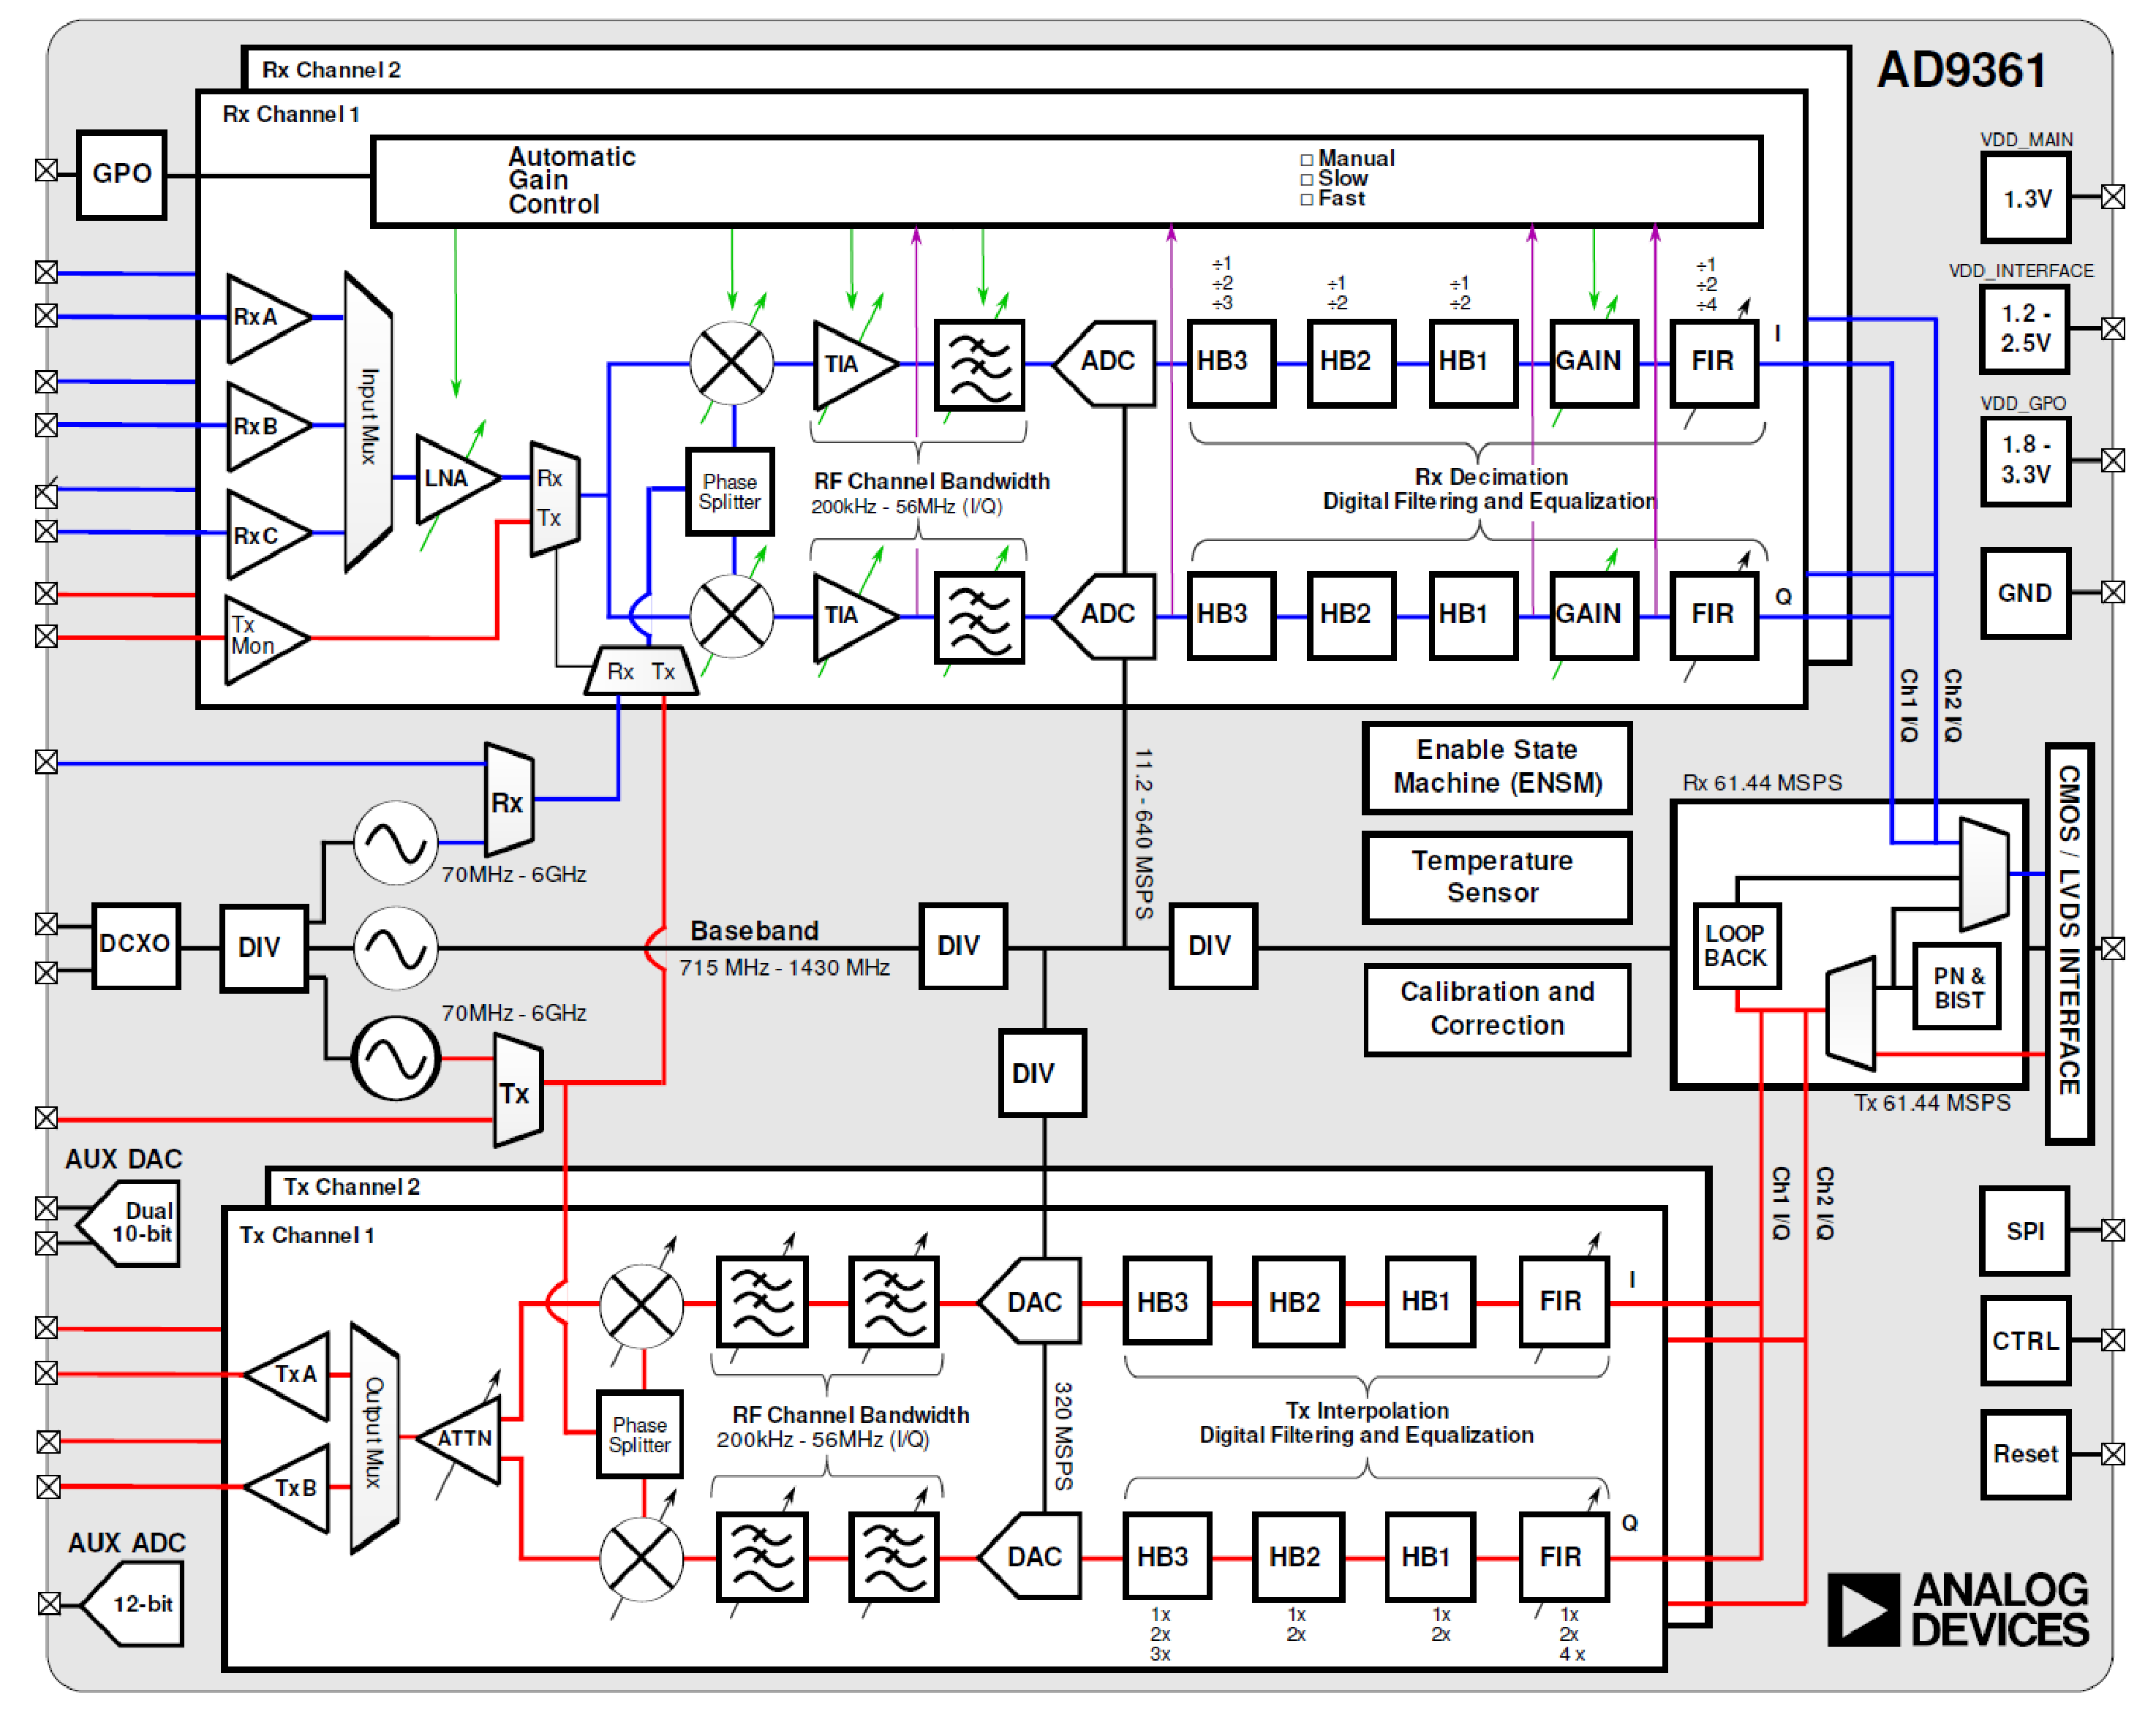
\includegraphics[width=0.65\textwidth]{./figures/ad9361_block_diagram}
    \caption{ AD9361 Block Diagram
    \label{fig:ad9361blk}}
\end{figure}

\subsection{Filtering}

In both receiver and transmitter there are:
\begin{description}
	\item[Receiver] \hfill \\
	\begin{itemize}
		\item Low pass filter : band shape to reduce adjacent-channel interference.
		\item Decimation Filter: up convert from the digital baseband rate (64.11MSPS max) to the actual ADC (640MSPS) rate.
	\end{itemize}
	\item[Transmitter] \hfill \\
\begin{itemize}
		\item Low pass filter : remove sampling artifacts
		\item Interpolation Filter : down convert from the digital baseband rate (64.11MSPS max) to the actual DAC (320MSPS) rate.
	\end{itemize}
\end{description}

In both digital and analog implementations these filters have impact the magnitude and the phase in passband, such behavior must be compensated in the system, and this compensation is usually done inside the 128-tap FIR filter. The FIR filter is not only used for low pass filter realization but also to compensate for magnitude and phase impacts created by the analog and digital half band filters in the desired baseband area. 

These filters depend in various other systems to work properly, such systems are sample rates, clock, data rates which sets the half band filters, and the desired RF bandwidth, which sets the analog filters. the process of loading a filter and after changing anything in the system will negatively affect the overall baseband performance. 

There is a filter too created by analog devices,which designs a low-pass filter and sets the FIR coefficients in order to ensure compensation for magnitude and phase changes in the analog or half band filters.

\subsection{Clocking}

%reescrever
The AD9361 has a series of internal PLL to generate and manipulate clock signals. There are fractional-n PLLs that generate the transmitter and receiver LO frequencies and there are the baseband PLL (BBPLL) used for the data converters, digital filters and I/O ports. All the frequency signals are generated using these PLLs clock outputs.

All the PLLs require a reference clock input and for this there is the digitally controlled oscillator (DXCO) function, which is an in-chip programmable and variable capacitor, such capacitor can tune the crystal frequency variance before entering the system, having a precision of +/- 6 ppm it results in a more accurate reference clock and can be used, if needed, for synchronization purposes. this function can also be used together with the on-chip temperature sensor to provide temperature compensation depending enviroment in which the chip will be used. For the reference clock there are two options:

\begin{description}
	\item[External Oscillator] \hfill \\
	In this option and external clock signal can be connected in the XTALP pin (Leaving the XTALP pin unconnected), this external clock frequency may vary from 10 MHz to 80 MHz. Such type of setup is needed when a wireless basestation (BTS) reference clock is locked to a master clock, and in such systems there is no or less need for clock synchronization.

	\item[Dedicated Crystal] \hfill \\
	In this option a dedicated crystal, with frequency varying from 19 MHz to 50 MHz, is connected in the XTALP and XTALN pins. This setup is usually used in wireless user equipment (UE), which do not need to be locked to a master clock but they do need to adjust periodically the LO frequency in order to maintain a connection with a BTS. The BTS periodically informs the UE of its frequency error relative to the BTS and the BBP can make adjustments to the reference clock and thus adjust the LO frequency if needed.

\end{description} 

\begin{figure}[htbp]
    \centering
    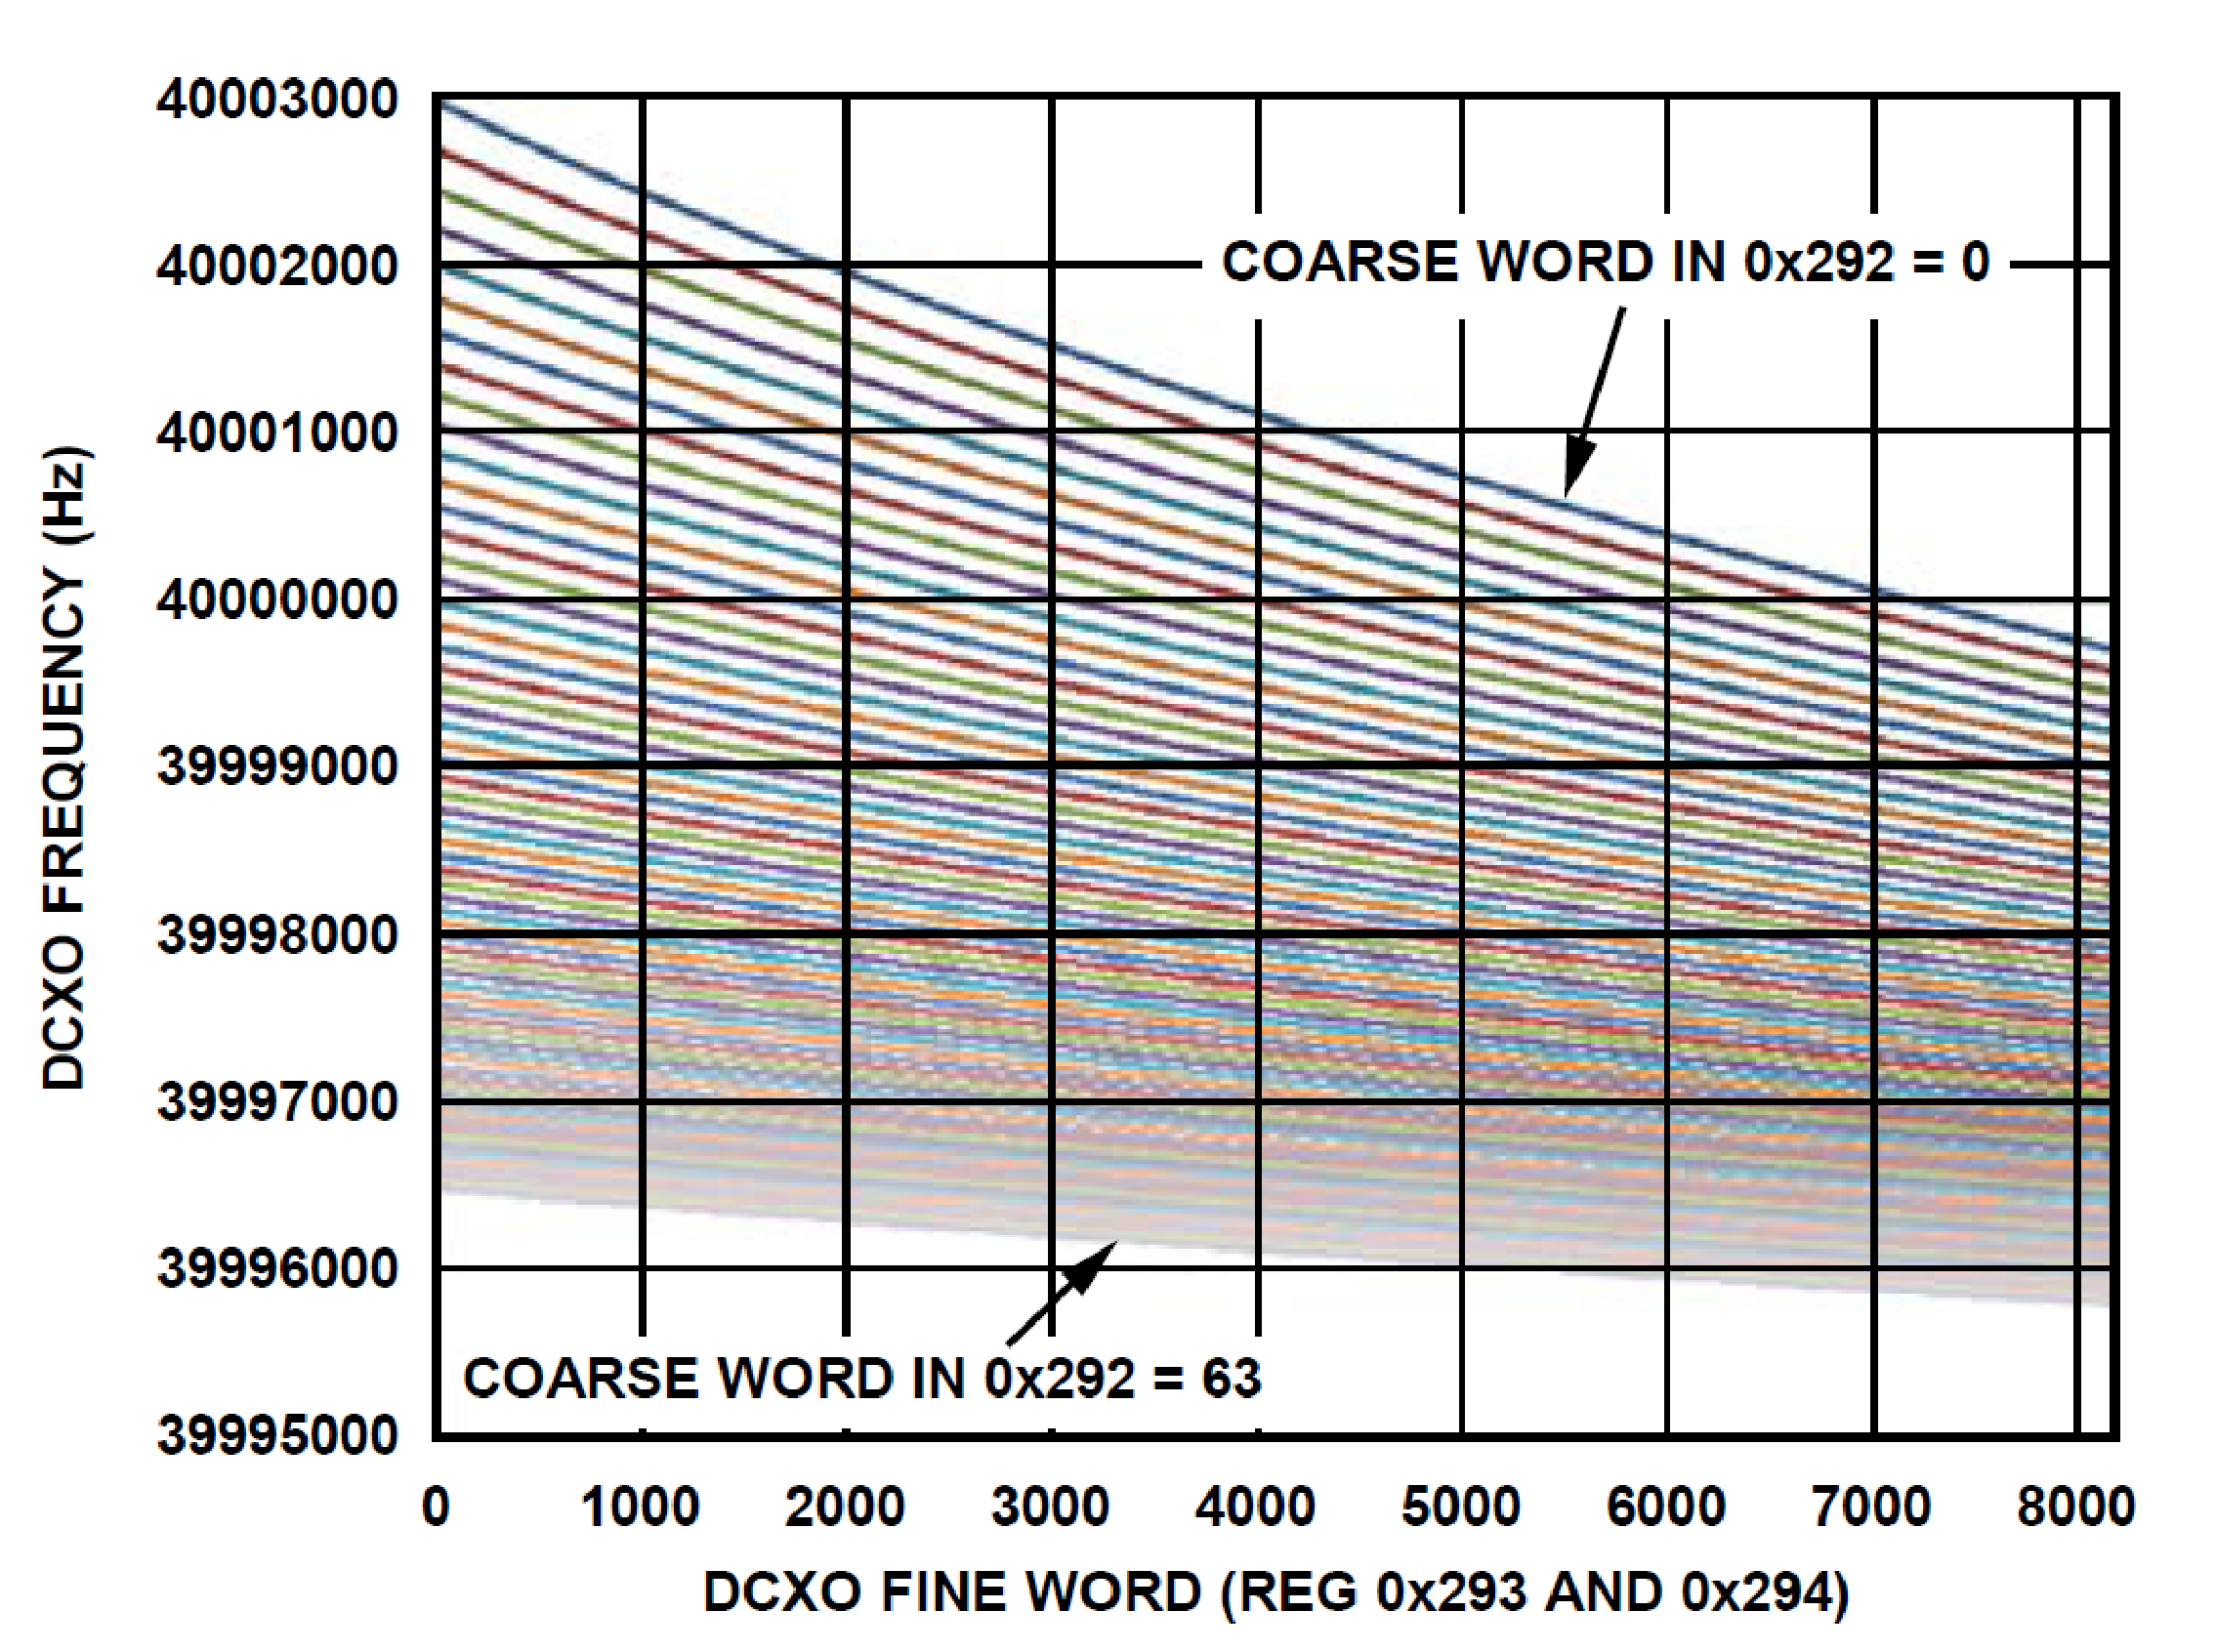
\includegraphics[width=0.65\textwidth]{./figures/dcxo_graph}
    \caption{ DCXO Behavior Graph
    \label{fig:pll}}
\end{figure}

\subsection{Synthesizers}

\begin{description}
	\item[RF PLLs] \hfill \\
	The AD9361 contains two identical synthesizers to generate the required LO signals for the RF signal path, one for the receiver and one for the transmitter. The PLL synthesizers are fractional-n PLLs with completely integrated VCOs and loop filters, requiring no other external components. In TDD operation mode, the synthesizers turn ON and OFF appropriate for the TX and RX frames, however in FDD TX PLL and RX PLL are activated at the same time.

	\item[BB PLL] \hfill \\
	The AD9361 contains also a baseband PLL synthesizer, which generate all the baseband related clock signals. The BBPLL feeds all the baseband related clock signals to ADC, DAC (Sampling Clock), DATA\_CLK signal and all data framing signals. This PLL has a frequency range from 700 Mhz to 1400 Mhz, and can be changed based on system requirements.

\end{description}

\begin{figure}[htbp]
    \centering
    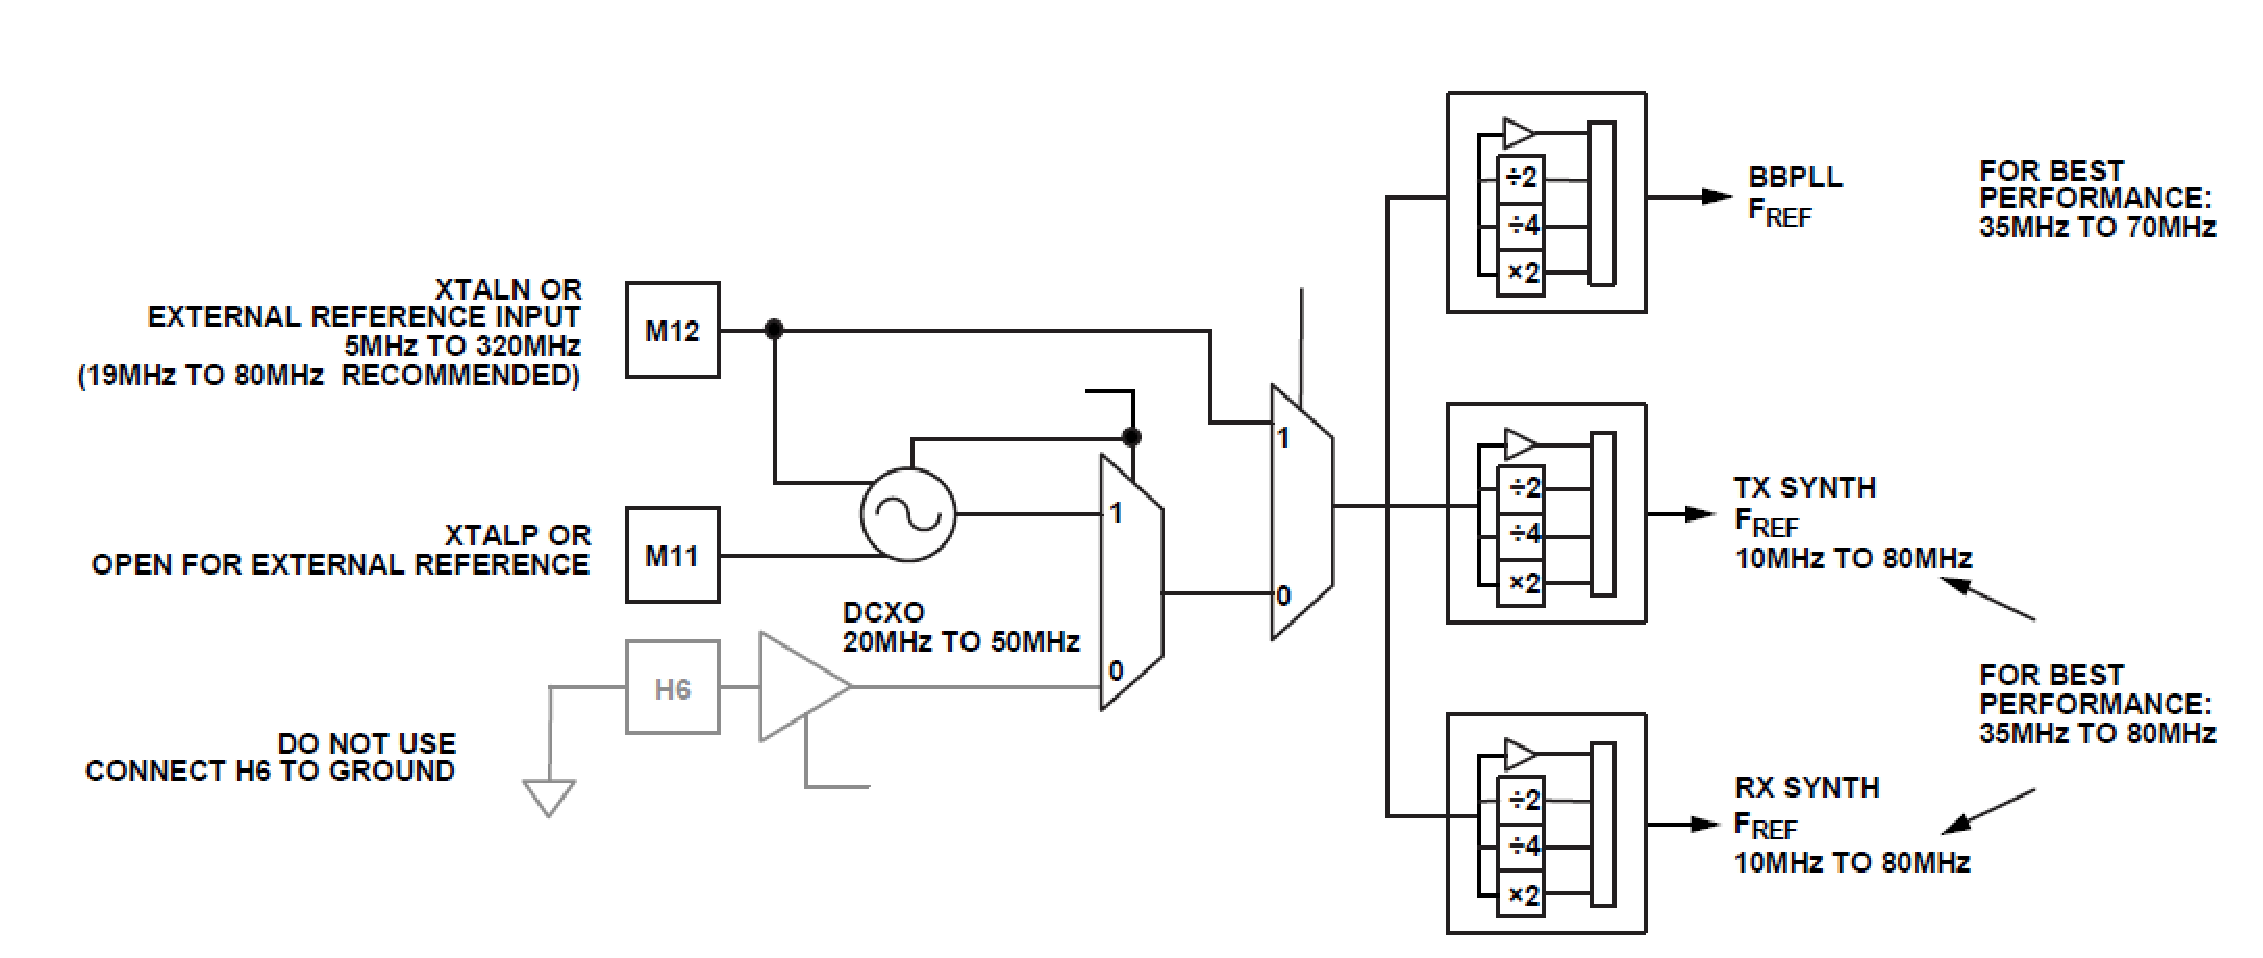
\includegraphics[width=0.65\textwidth]{./figures/pll_ref_block}
    \caption{ AD9361 PLL Reference Block Diagram
    \label{fig:pll}}
\end{figure}

\subsection{Digital Data Interface}

The AD9361 uses parallel data ports to transfer data between the device and the BBP. These data ports can be configured either single-ended CMOS format or LVDS format (used in this work). Both formats can be configured in multiple arrangements to adequate the system requirements for data transfer and connections. These arrangements can be of single port data bus, dual port data bus, single data rate, double data rate and other various combinations compatible with the device.\\
Bus transfers are controlled using hardware handshake signalling, these two ports can be operated in TDD (bidirectional) or FDD (full duplex) where half of the bits are used for transmitting and the other half is used for receiving. The interface can also be configured to use only one of the data ports ( usually used in applications that do not require high data rates or samples).\\
The communication between the BBP processor and the AD9361 rely on some signals to properly work, which are DATA\_CLK, FB\_CLK and RX\_FRAME, its operation is detailed below:

\begin{description}
	\item[DATA\_CLK Signal] \hfill \\
	RX sends the signal DATA\_CLK to the BBP, which can be used when receiving data. DATA\_CLK can be used to control data sampling time, which can be single data rate (data is captured on rising clock edge) or double data rate (data is captured on both rising and falling clock edges). This can be applied using single or dual data port.

	\item[FB\_CLK Signal] \hfill \\
	The FB\_CLK signal must have the same frequency and duty cycle as DATA\_CLK and like DATA\_CLK it is used as timing reference for the interface. FB\_CLK allows source synchronous with rising edge capture for burst control signals and can be used like DATA\_CLK for rising edge, single data rate mode or in both edge capture, double data rate mode for transmit signal bursts.

	\item[RF\_FRAME Signal] \hfill \\
	The RF\_FRAME signal is generated by the device whenever the receiver outputs valid data. RF\_FRAME has two modes:
	\begin{itemize}
		\item \textbf{Level Mode:} RF\_FRAME stays high as long as the data is valid.
		\item \textbf{Pulse Mode:} RF\_FRAME pulses with 30% duty cycle.
	\end{itemize}
	The BBP must provide a TX\_FRAME that indicates beginning of a valid data transmission with a rising edge. The TX\_FRAME operates similarly as the RF\_FRAME, on Level Mode or Pulse Mode.

\end{description}

\begin{figure}[htbp]
    \centering
    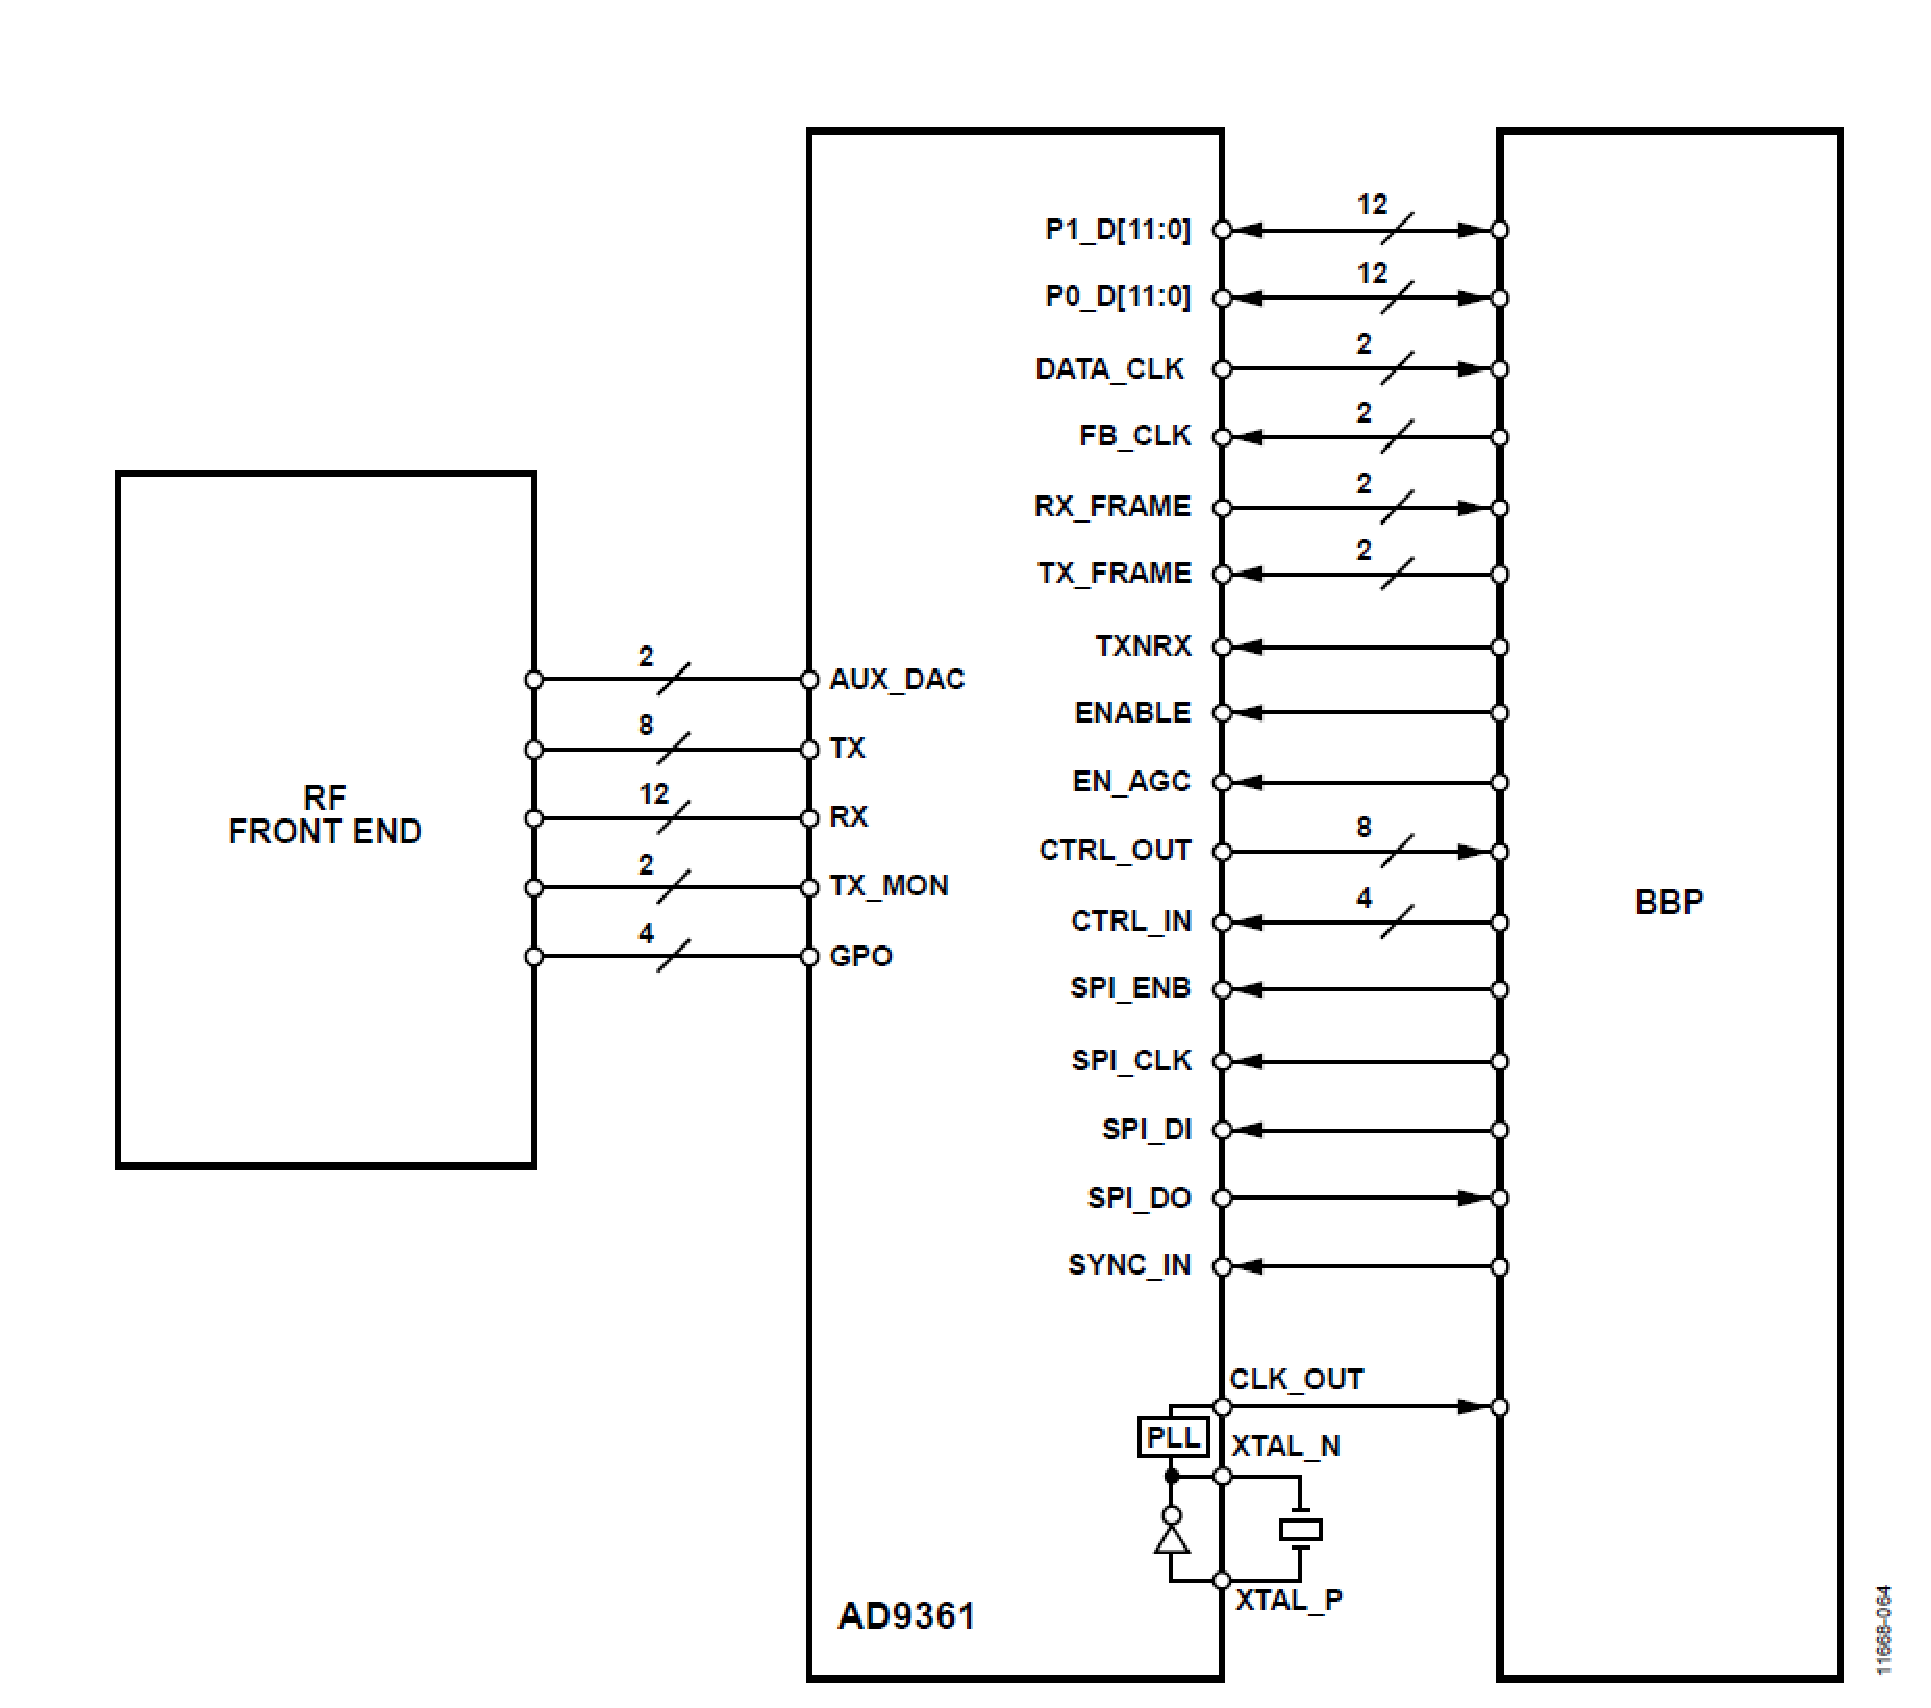
\includegraphics[width=0.65\textwidth]{./figures/ad9361_digital_interface}
    \caption{ AD9361 Digital Data Interface
    \label{fig:ad9361diginterface}}
\end{figure}


\subsection{Enable State Machine}

The AD9361 has an Enable State Machine (ENSM) which allows real-time control over the current state of the device. The device can be place in several states like:

\begin{itemize}
		\item \textbf{Wait:} Power save, synthesizers disabled.
		\item \textbf{Sleep:} Wait with all clocks and BBPLLs disabled.
		\item \textbf{TX:} TX chain enabled.
		\item \textbf{RX:} RX chain enabled.
		\item \textbf{FDD:}TX and RX chains enabled.
		\item \textbf{Alert:} Synthesizers enabled.
	\end{itemize}
	This ENSM can be controlled either by SPI or PIN (GPIO for example), where the SPI control mode is for a non real-time operation and the PIN control mode is for a much faster and real-time control.
	

\begin{description}
	\item[SPI Control Mode] \hfill \\
	In SPI control mode, the BBP writes registers asynchronously by using SPI protocol to access the addresses, and by writing these registers the state machine advances the current state to the next state. SPI communication is considerece asynchronous to the DATA\_CLK because the SPI\_CLK can be derived from another clock source, where BBP and the device does not share the same clock source. This control method is recommended when there is no need for a real-time control.

	\item[Pin Control Mode] \hfill \\
	In Pin control mode, there are pins dedicated to activate some states of the ENSM, like ENABLE pin and TXNRX pin, this mode allows a real-time control of the current state. This method is recommended in a system where the BBIC has extra pins to spare with the real-time control outputs, this 2-wire interface can control the state of the device.
	To advance the current state to the next state of the ENSM, the enable function of the ENABLE pin can be driven by either pulse or level,if the pulse is used the minimum width of the pulse needs to be equal as the FB\_CLK cycle.
	In FDD mode, the ENABLE and TXNRX pins can be remapped to be used as real-time control of the TX and RX data transfers. In this mode ENABLE enables or disables the receive signal and TXNRX enables or disables the transmit signal, using such mode  causes the ENSM to be removed from the system for data flow control and is replaced by these pins.

\end{description}

\begin{figure}[htbp]
    \centering
    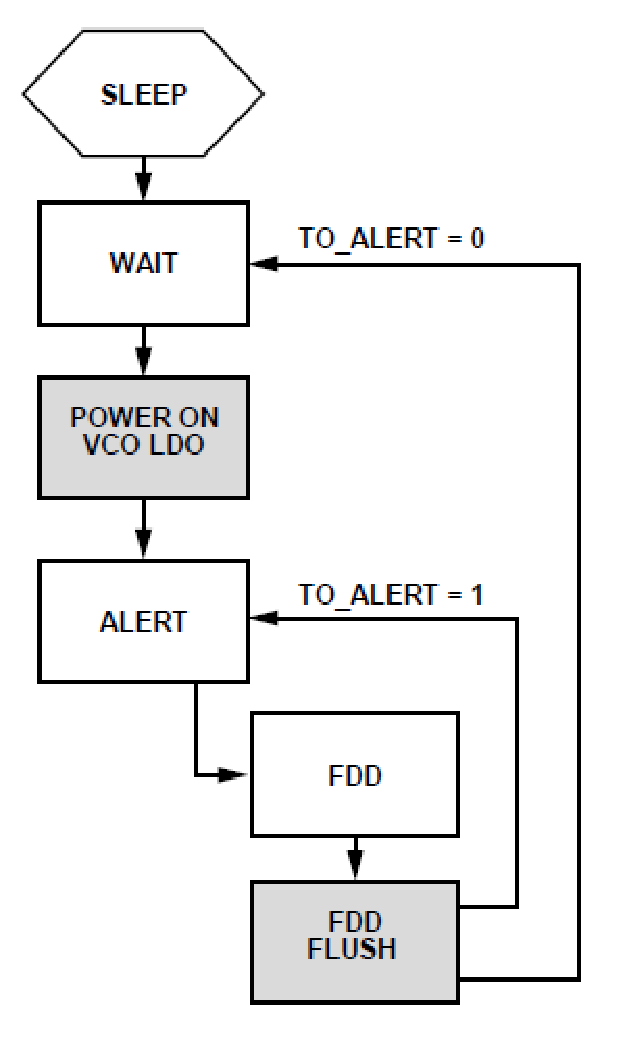
\includegraphics[width=0.65\textwidth]{./figures/fdd_ensm}
    \caption{ FDD Enable State Machine
    \label{fig:pll}}
\end{figure}

\begin{figure}[htbp]
    \centering
    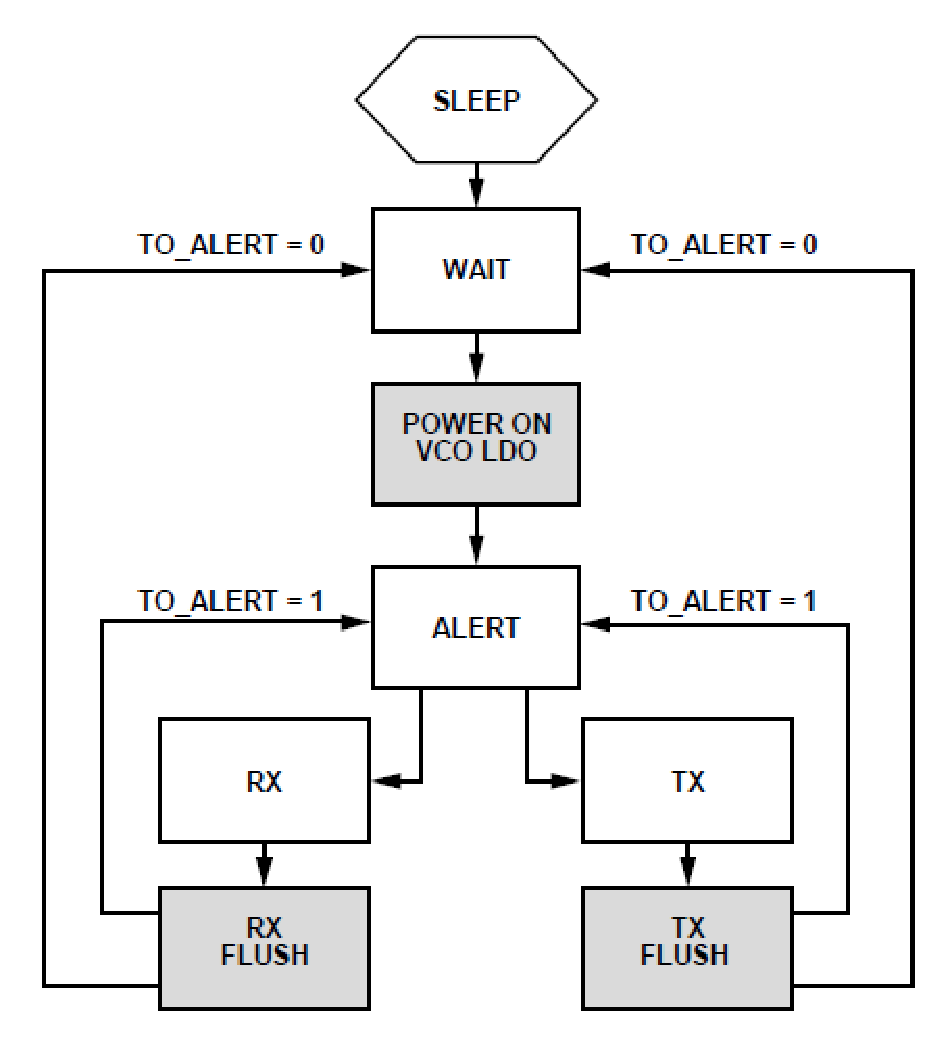
\includegraphics[width=0.65\textwidth]{./figures/tdd_ensm}
    \caption{ TDD Enable State Machine
    \label{fig:pll}}
\end{figure}


\subsection{SPI Interface}

The AD9361 uses a SPI interface for communication with the BBP. Throught SPI is possible to access all the device registers. The PSI interface can be configured as a 4-wire interface with dedicated transmit and receive pins, duplex, or as 3-wire interface with bidirectional data port. 
Write commands have a 24-bit format where the first six bits are for setting the bus direction and number of bytes to transfer, the next 10 bits set the address where the data is to be written and the final eight bits are the data to be transferred to the specific register address (MSB to LSB), a LSB-first format is also supported.
Read commands follow a similar format, the difference is that the first 16 bits are transferred on the SPI\_DI pin and the final eight are read from the AD9361, either using SPI\_DO (4-wire interface) or SPI\_DI (3-wire interface).

\subsection{Auxiliary Converters}

\begin{description}

	\item[AUXADC] \hfill \\
	The AD(361 contains an auxiliary ADC that can be used to monitor some system functions such as temperature or power output, it is a 12-bit converter and has an input range of 0V to 1.25V. The SPI can read the last value latched at the output of the ADC when it is enabled for use, there is also a multiplexer that permits to select between AUXADC and built-in temperature sensor.

	\item[AUXDAC1 and AUXDAC2] \hfill \\
	The AD(361 also has two identical auxiliary DACs which can be used to provide power amplifier (PA) bias or other system functionality. Both the DACs are 10-bit wide and have an output range of 0.5 V to 0.3V and have a current drive of 10mA. The DACs can be directly controlled by the ENSM.

\end{description}

\subsection{Applications}


\section{FMCommS2}

FMCommS2 is basically evaluation board for the AD9361 that has a FPGA Mezzanine Card (FMC) connector for interfacing with the BBP (Usually FPGA). The FMComms2 has 5 SMA connectors, 2 for Rx, 2 for Tx and one for external reference clock input. The FMComms2 provides a 2x2 RF configuration, extended from the AD9361, and has  a narrow tuning range balun, which is performance optimized for 2.4GHz.
The FMComms2 is a transceiver intended for use in RF applications such 3G or 4G BTS or SDR. Its programmability and wideband capability make it ideal for broad range of transceiver applications and make it very attractive for the new C-RAN paradigm.

\begin{figure}[htbp]
    \centering
    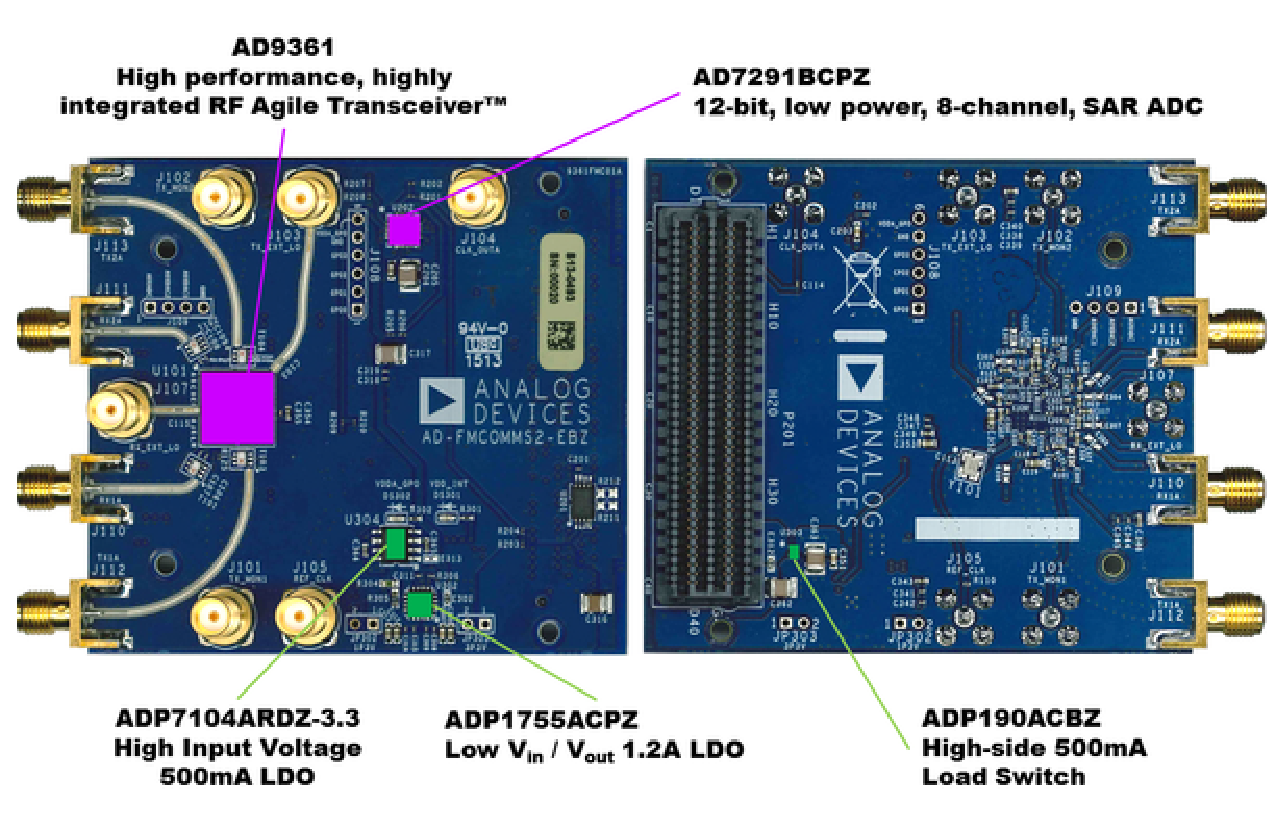
\includegraphics[width=0.65\textwidth]{./figures/fmcomms2_pic}
    \caption{ FMComms2 and its components
    \label{fig:fmcomm}}
\end{figure}


\subsection{Functional Overview}

The Block diagram show that there are 4 main functional partitions - receiver path, transmit path, clocking and power supply. Since the FMComms2 incorporates and extends the basic functionalities of the AD9361, thus the data path is fully integrated into the AD9361.

\begin{figure}[htbp]
    \centering
    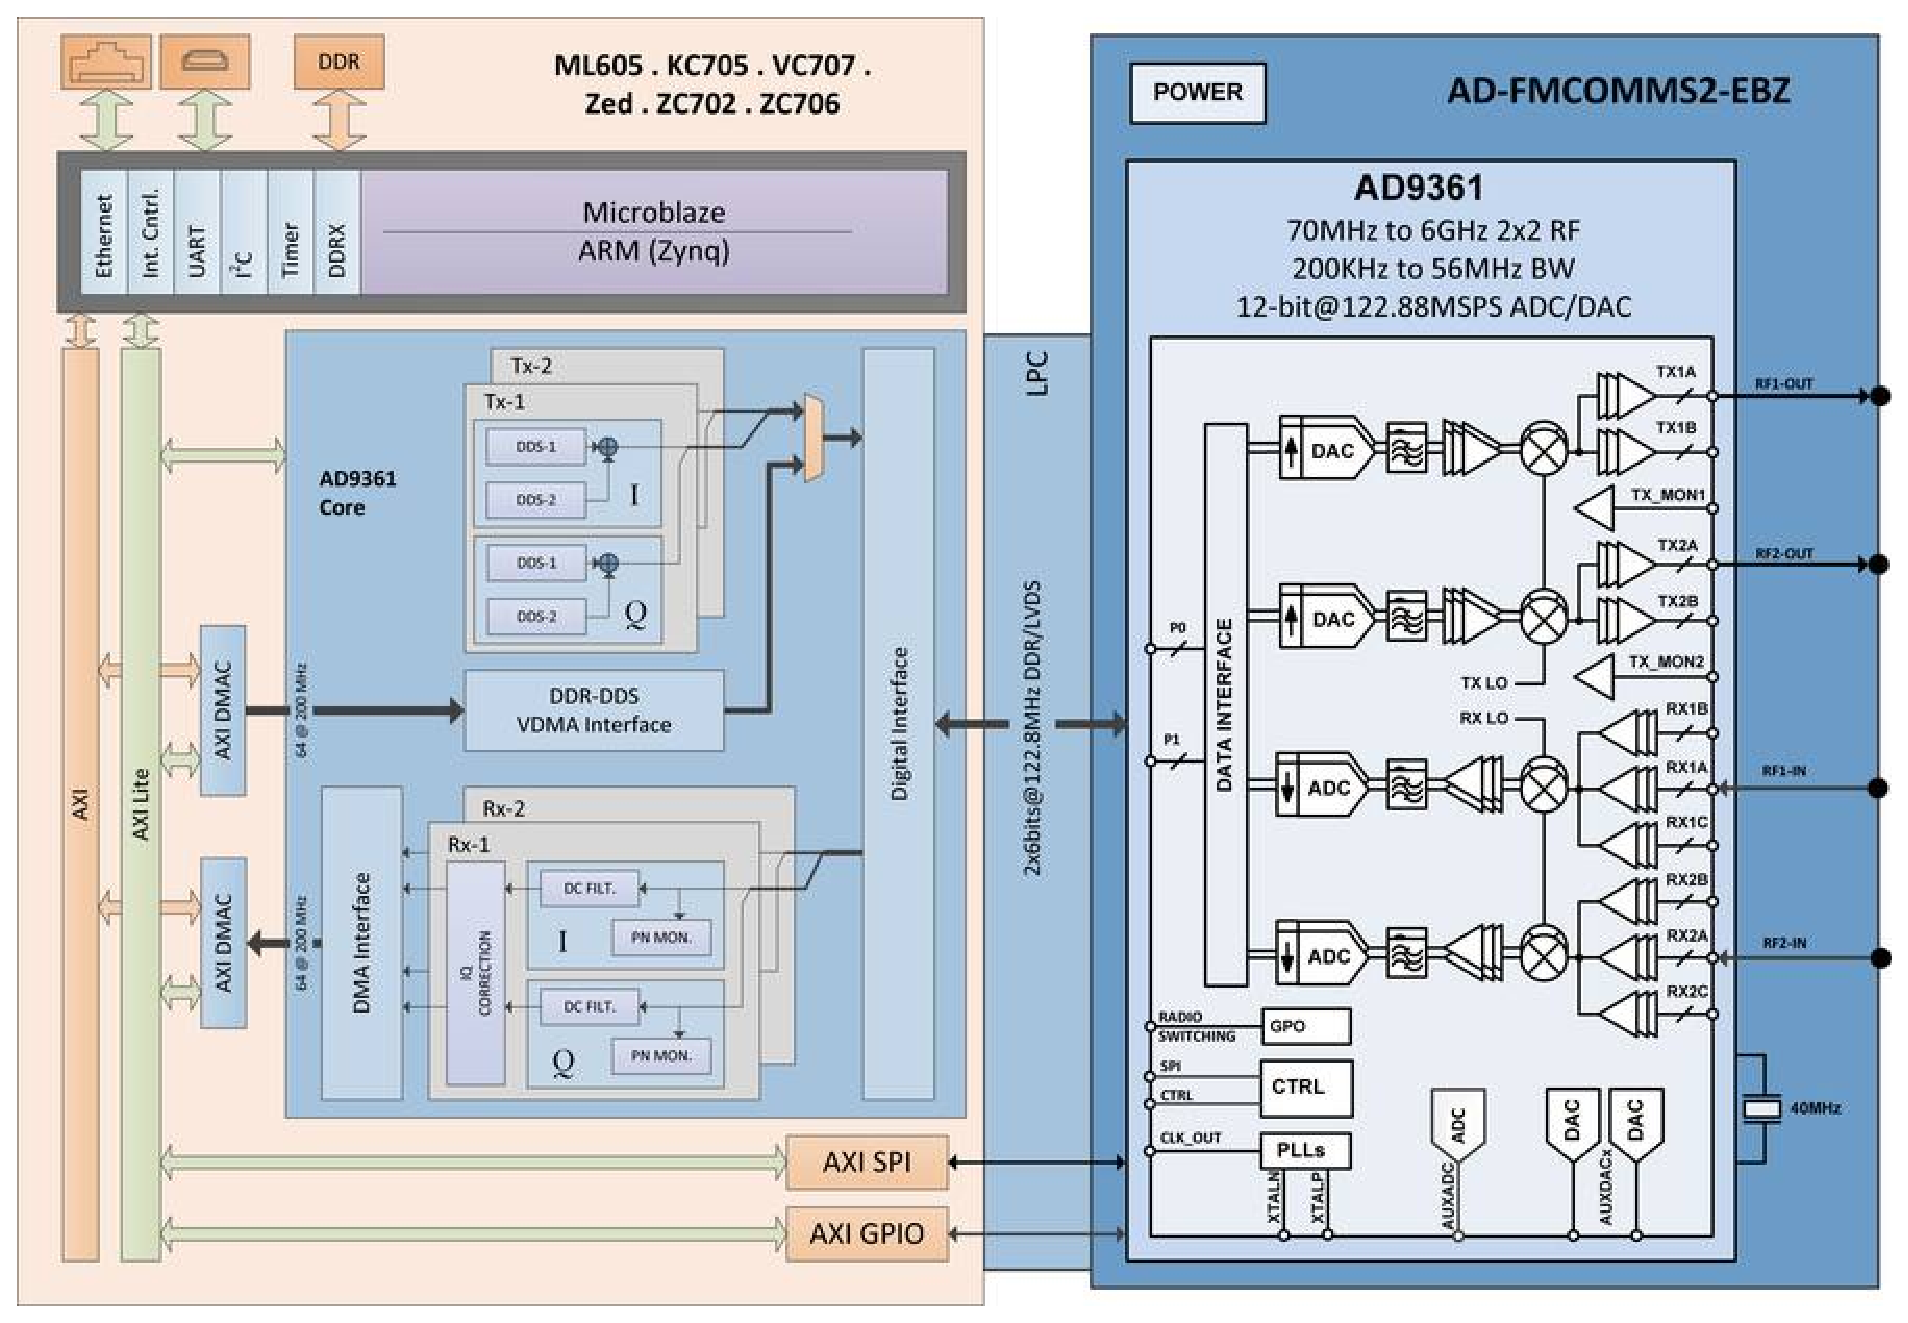
\includegraphics[width=0.65\textwidth]{./figures/fmcomms2_bd}
    \caption{ FMComms2 and FPGA Block Diagram
    \label{fig:fmcommbd}}
\end{figure}



\begin{description}
	\item[Receive] \hfill \\
	\begin{itemize}
		\item Support up to 2 direct conversion RF receiver channels.
		\item Fully integrated frequency synthesizers (including loop filter).
		\item Data path consists in LNA, Demodulator, LPF, ADC and digital filters.
		\item \textit{AGC:} quadrature calibration and DC offset calibration.
		\item \textit{NF:} 2.5 dB at 1Ghz.
		\item \textit{ADC:} Continuous time sigma-delta ( $\Sigma - \Delta$), 640 MSPS.
		\item \textit{Digital FIlter:} 128 COmplex taps with decimation between 2 and 48.
		\item \textit{Gain:} 1dB step size, 80 dB analog Range, 30 db digital range (post ADC scaling).
		\item On-chip sensor for temperature corrected RSSI.
	\end{itemize}

	\item[Transmit] \hfill \\
\begin{itemize}
		\item Supports up to 2 direct conversion RF transmit channels.
		\item Fully integrated frequency synthesizers (including loop filter).
\item Data path consists of digital filters, DAC and modulators.
		\item \textit{Digital FIlter:} 128 complex taps with interpolation between 2 and 48.
		\item \textit{Gain:} 0.5 dB step size, 86 dB range.
		\item \textit{ADC:} 340 MSPS.
	\end{itemize}

	\item[Clocking] \hfill \\
		The FMComms2 board has a integrated crystal oscillator of 40 Mhz and has a SMA input for external clock input.

	\item[Control/Monitor] \hfill \\
		The board allows real time control and monitoring via dedicated pins, such pins functionality are programmable. The control and monitor programming configuration is specified in the ad9361 section \cite{sec:ad9361}.

\end{description}

\section{Basic Mathematical Background}

\subsection{Complex Modulation}

\begin{eqnarray}
	I = sin(\omega \times t)\\
	Q = cos(\omega \times t)
\end{eqnarray}

\begin{equation}
	cos(\omega \times t) = sin(\frac{\pi}{2} - (\omega \times t))
\end{equation}

then:

\begin{eqnarray}
	I = sin(\omega \times t)\\
	Q = sin(\frac{\pi}{2} - (\omega \times t))
\end{eqnarray}

These are the two signals coming out of the DAC, two sine waves, phase offset from each other, wich is called IQ.

\subsection{Basic Modulation Mathematics}

Start to modulating signal from a amplitude perspective:

\begin{eqnarray}
LO_I = A_x cos(k)\\
LO_Q = B_x sin(k)
\end{eqnarray}

We still have the carrier:

\begin{equation}
LO_I = cos(\omega) ; LO_Q = sin(\omega)
\end{equation}

Will result:

\begin{eqnarray}
LO_I \times I = A_x cos(k) \times sin(\omega)\\
LO_Q \times I = B_x sin(k) \times cos(\omega)
\end{eqnarray}


That gives the output:

\begin{equation}
x(t)=A_x cos(k)\times sin(\omega)+ B_x sin(k)\times cos(\omega)
\end{equation}

This does not match with any trigonometrical identities and it is easier to use Euler\'s formula:

\begin{eqnarray}
sin(x)=(\frac{1}{2}e^{-jx} - \frac{1}{2}e^{jx})\\
cos(x)=(\frac{1}{2}e^{-jx} + \frac{1}{2}e^{jx})
\end{eqnarray}

Therefore:

\begin{equation}
x(t)=A_x (\frac{1}{2}e^{-jk} + \frac{1}{2}e^{jk})\times (\frac{1}{2}e^{-j\omega} - \frac{1}{2}e^{j\omega})+ B_x (\frac{1}{2}e^{-jk} - \frac{1}{2}e^{jk})\times (\frac{1}{2}e^{-j\omega} + \frac{1}{2}e^{j\omega})
\end{equation}

\begin{equation}
x(t)=\frac{A}{2} (e^{-jk} + e^{jk})\times (e^{-j\omega} - e^{j\omega})+ \frac{B}{2} (e^{-jk} - e^{jk})\times (e^{-j\omega} + e^{j\omega})
\end{equation}

If we expand we get:

\begin{equation}
x(t)=\frac{1}{2} ((Ae^{-jk-j\omega} + Ae^{jk-j\omega} - Ae^{-jk+j\omega} - Ae^{jk+j\omega}) + (Be^{-jk-j\omega} - Be^{jk-j\omega} - Be^{-jk+j\omega} + Be^{jk+j\omega}))
\end{equation}


And then:

\begin{equation}
x(t)=\frac{1}{2} ((A+B)e^{-jk-j\omega} + (A-B)e^{jk-j\omega} - (A-B)e^{-jk+j\omega} - (A+B)e^{jk+j\omega})
\end{equation}

It is possible to rearrange as:

\begin{equation}
x(t)=\frac{1}{2} \times ((A+B)(e^{-jk-j\omega} - e^{jk+j\omega}) + (A-B)(e^{jk-j\omega} - e^{-jk+j\omega}))
\end{equation}

And then:

\begin{equation}
x(t)=(\frac{A+B}{2} )(sin(k+\omega)) + (\frac{A-B}{2} )(sin(k-\omega))
\end{equation}

If this due to amplitude mismatch, this creates an image on the other side of the local oscillator.





\chapter{FPGA}
\section{ML605 - Virtex6}
\section{VC707 - Virtex7}

\chapter{Setup Description}


\section{Overview}

\section{Integration between FPGA and FMComms2}

\part{Final Results}
\chapter{Results}

\section{Preliminary Tests}

\section{Transmission Tests}


\part{Conclusion and Future Work}
\chapter{Conclusion}
\label{chap:conclusion}

\section{Conclusion}
\label{sec:conclusion}

The development of this setup was meant to be general and be used in both
research and academic environments. The process of implementing this setup went
through a myriad of fields in telecommunications and embedded systems, such as
communication protocols, embedded programming, electronics and many others,
being this setup a testbed for more complex processes inside the LTE band saves
a lot of time in development. \\

The FMComms2 board allows real-time and scalable change in parameters by
software or hardware signals, and it re-calibrates and reconfigures itself if
needed so, which makes a very good transceiver board to be used in a C-RAN
environment.\\

This setup was extensively documented and can be used in digital communication
classes to show how a real radio frontend system is made, of course there is
much to improve, there is no dynamic clock synchronization between the FPGA and
the FMComms2, there is no communication protocol between the FPGA (BBP) and the
external world other than the FMComms2 such things are necessary to have a real
frontend but were outside the scope of this project which was just to evaluate a
setup for a scalable and dynamically configurable frontend.\\

Although the FMComms2 and the FPGA operates on different clocks, thus no real
synchronization was implemented, this setup has the minimal capability of
transmitting and receiving signals and reconfigure itself on real-time, the main
goal of this work was reached, however there is much to explore with these tools
and devices.

\section{Future Works}
\label{sec:futurew}

Having finished this part of the work a natural sequel would be implementing
Ethernet connection driver in the FPGA, making it possible to receive data from
Ethernet and hand this to the transceiver board following the schematic on
figure \ref{fig:setupeth} idea. This would be a challenge because there is a lot
of things to consider, but the most problematic of them all is synchronization,
the clock in which everything inside the FPGA works is different from the AD9361
clock not only in frequency but in phase, this can bring a lot of problems,
however there is the possibility of feeding FMComms2 with an external clock
which would increase its performance.\\

With Ethernet it would be possible to generate the modulated samples and send
them trough air, just like Gnuradio + USRP and thus demodulate the received back
samples in the PC, however there is another possibility, modulation and
demodulation blocks implemented in the FPGA logic, thus much faster than the PC
ones and with partial reconfiguration there is the advantage of loading various
schemes of modulation/demodulation in the FPGA, implementing thus a very good
SDR. The Ethernet connection, is also very interesting for C-RAN
environment, because Ethernet is cheap and easy to implement.\\

\begin{figure}[htbp]
    \centering
    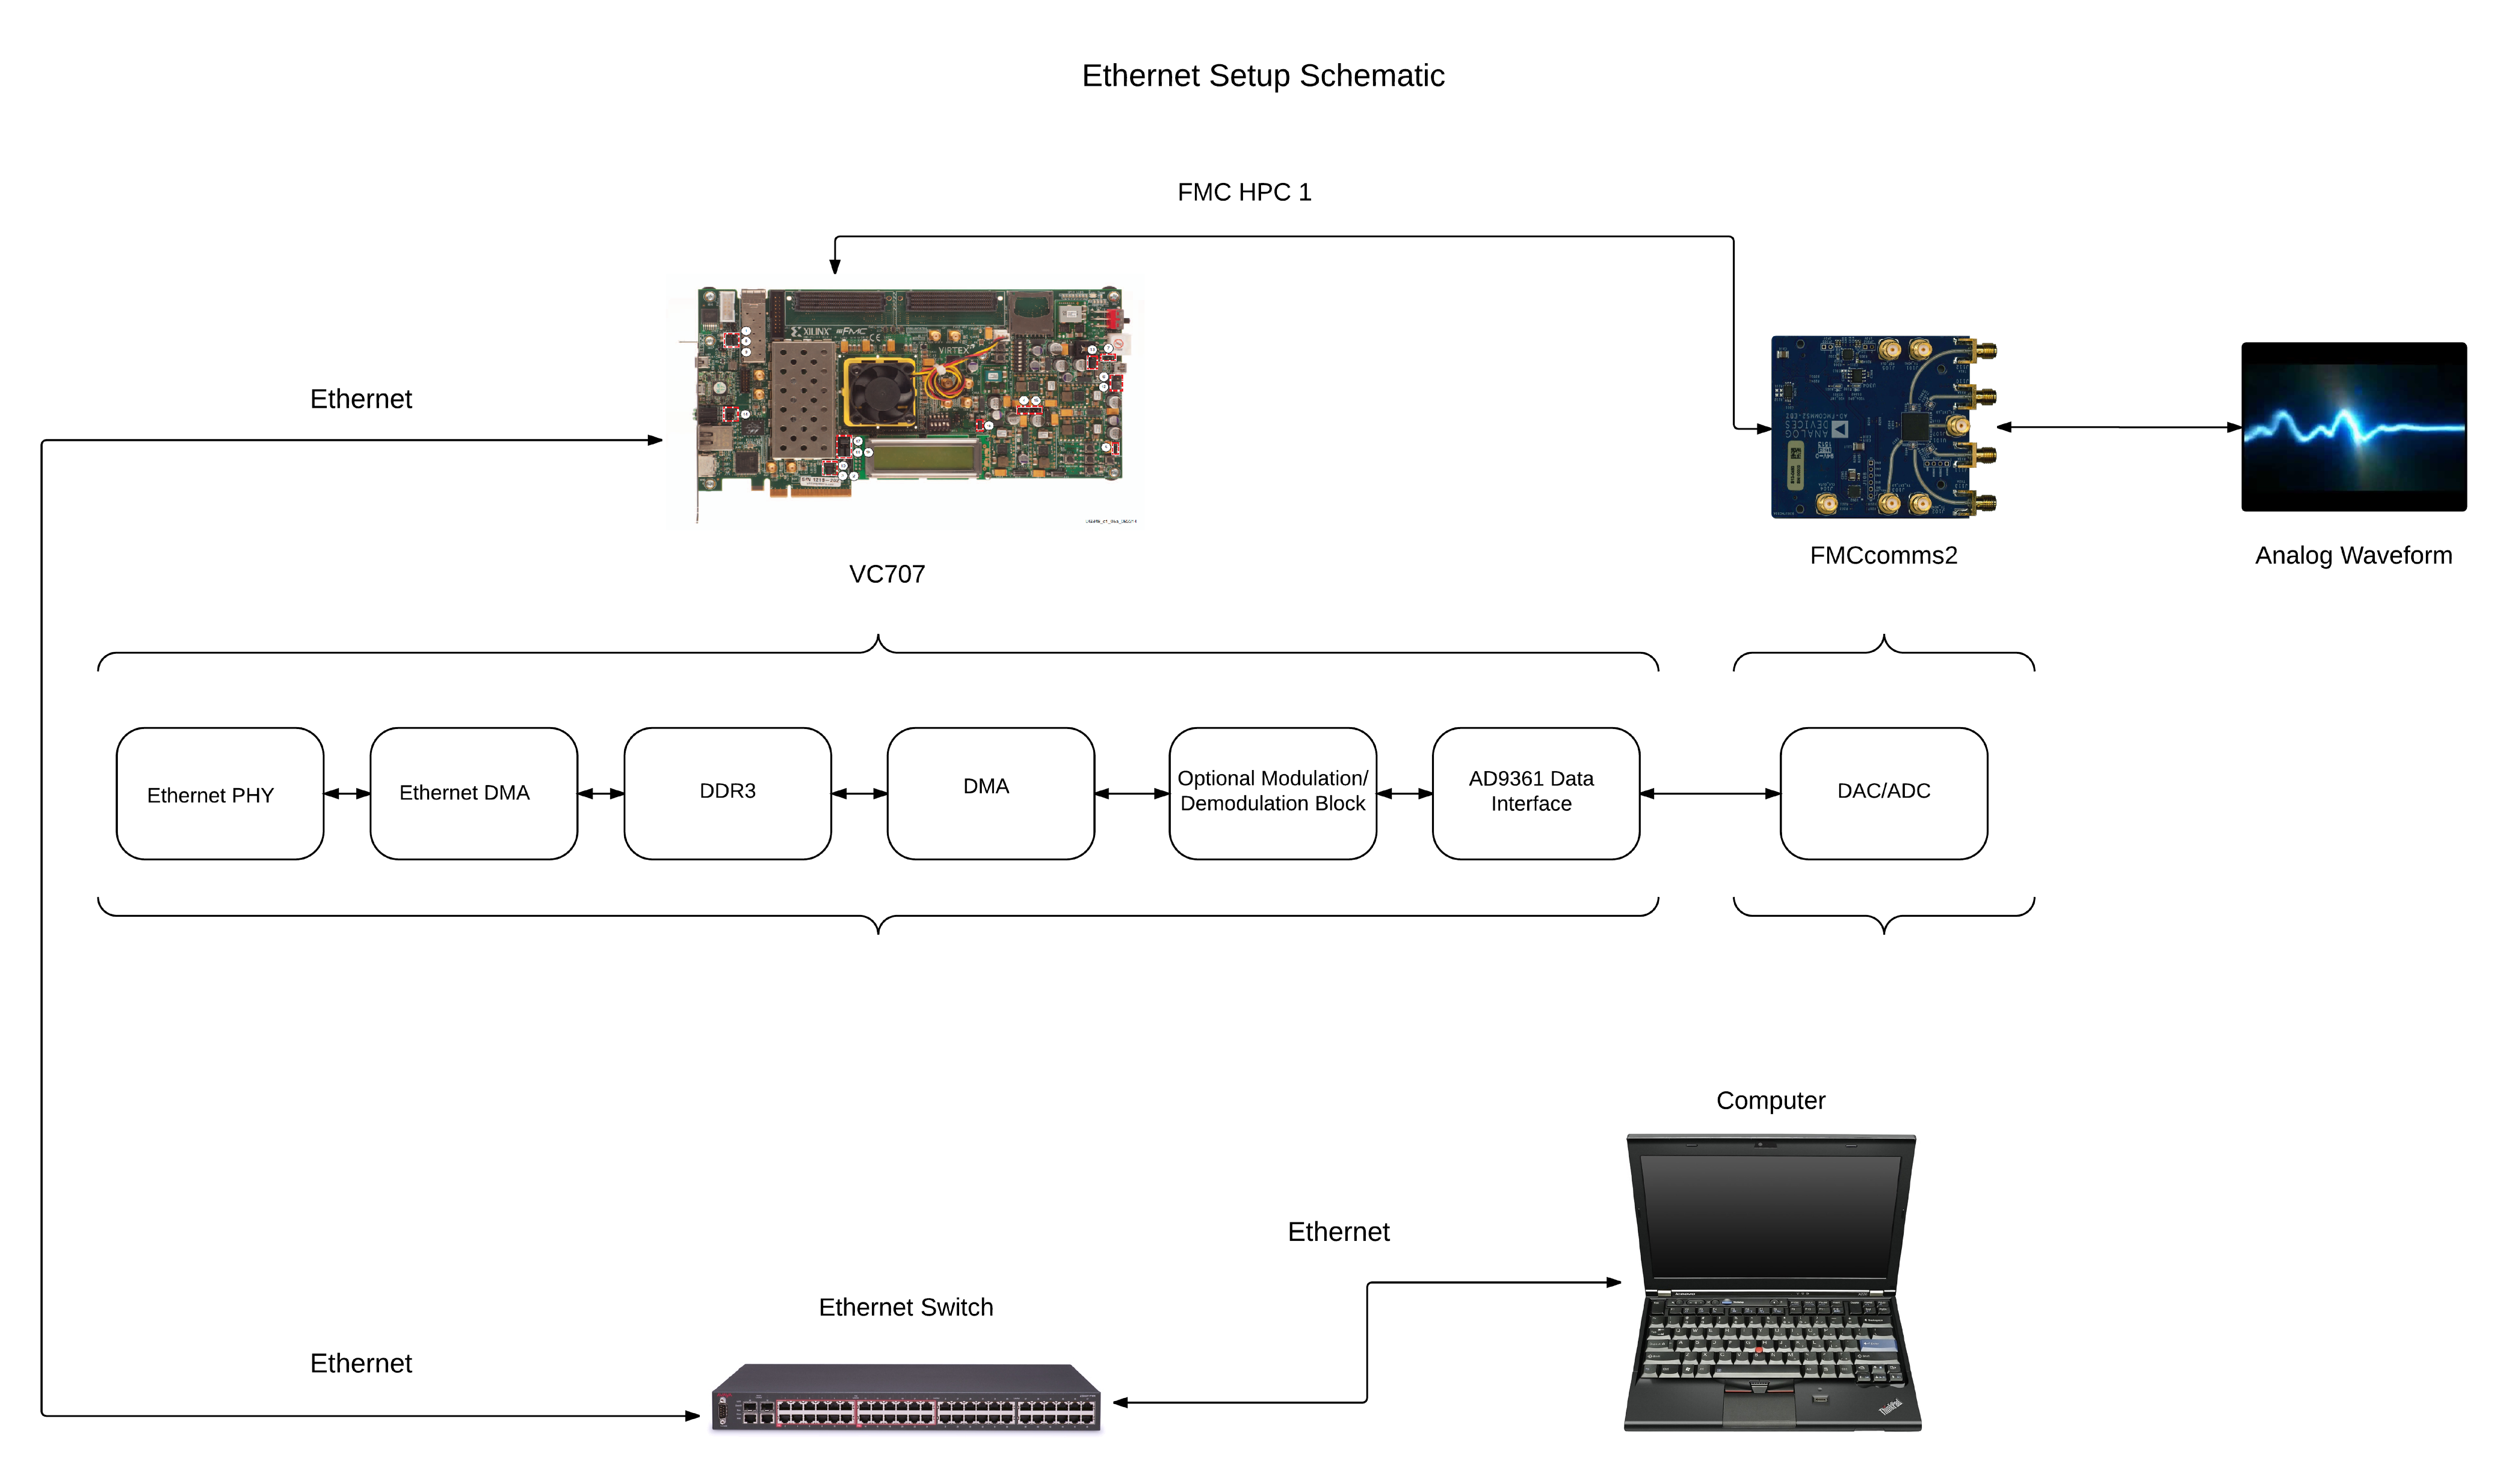
\includegraphics[width=0.65\textwidth]{./figures/eth_setup}
    \caption{ Setup Enhanced with Ethernet Connection
    \label{fig:setupeth}}
\end{figure}


%%%%%%%%%%%%%%%%%%%%%%%%%%%%%%%%%%`
%   Referencias bibliograficas   %
%%%%%%%%%%%%%%%%%%%%%%%%%%%%%%%%%%

\renewcommand\bibname{Refer�ncias Bibliogr�ficas}
%\bibliographystyle{../../../public/ABNT-20020112}
%\bibliographystyle{../public/IEEEtran}
%\bibliographystyle{../../../Public/IEEEtran_pt}
\bibliographystyle{abnt}
\bibliography{references}

%temorary tag just while there is no \citation
%eliminates no \citation error
\nocite{*}

\clearpage

%%%%%%%%%%%%%%%%%%%%%
%   Apêndices    %
%%%%%%%%%%%%%%%%%%%%%

\appendix
\chapter{PLL}
\chapter{FPGA Design Flow}
\chapter{AD9361 NO-OS Driver}


%%%%%%%%%%%%%%%%%%%%%
%   Página em branco    %
%%%%%%%%%%%%%%%%%%%%%

\newpage
\thispagestyle{empty}
\mbox{}

%% -- Termino do TCC
\end{document}
